%%%%%%%%%%%%%%%%%%%% book.tex %%%%%%%%%%%%%%%%%%%%%%%%%%%%%
%
% sample root file for the chapters of your "monograph"
%
% Use this file as a template for your own input.
%
%%%%%%%%%%%%%%%% Springer-Verlag %%%%%%%%%%%%%%%%%%%%%%%%%%


% RECOMMENDED %%%%%%%%%%%%%%%%%%%%%%%%%%%%%%%%%%%%%%%%%%%%%%%%%%%
\documentclass[graybox,envcountchap,sectrefs]{svmono}

% choose options for [] as required from the list
% in the Reference Guide

\usepackage{mathptmx}
\usepackage{helvet}
\usepackage{courier}
%
\usepackage[utf8]{inputenc}
\usepackage{type1cm}         

\usepackage{makeidx}         % allows index generation
\usepackage{graphicx}        % standard LaTeX graphics tool
                            % when including figure files
\usepackage{svg}
\usepackage{multicol}        % used for the two-column index
\usepackage[bottom]{footmisc}% places footnotes at page bottom
%
\usepackage{pgfplots}
\pgfplotsset{compat=1.13}%\pgfplotsset{compat=1.14}
\pgfkeys{/pgf/number format/.cd,1000 sep={\,}}
%----- Bibliografia ------------
\usepackage[style=mexican]{csquotes}
\usepackage[backend=biber, style=authoryear]{biblatex}% biber
\addbibresource{ReferenciasMulti.bib}
\usepackage{emptypage}
%% ********* Table layout **************
\usepackage{booktabs}
\usepackage{multirow}
\usepackage{tabularx}
\usepackage{tabulary}
\usepackage{tcolorbox}
% see the list of further useful packages
% in the Reference Guide
%% Math Packages %%%%%%%%%%%%%%%%%%%%%%%%%%%%%%%%%%%%%%%%%%%%
\usepackage{amsmath}
\usepackage{textcomp}
%\usepackage{amsthm}
\usepackage{amsfonts}
\usepackage{bm}  %pone en negrita letras griegas
%
\usepackage[nogroupskip, nonumberlist, acronyms]{glossaries}%
\makeglossaries
%
\graphicspath{{./figuras/}}
\svgpath{{./figuras/}}
\pdfsuppresswarningpagegroup=1
\newcommand{\xv}{\mathbf{x}}
\newcolumntype{K}[1]{>{\centering\arraybackslash}p{#1}}

\makeindex             % used for the subject index
                       % please use the style svind.ist with
                       % your makeindex program

%%%%%%%%%%%%%%%%%%%%%%%%%%%%%%%%%%%%%%%%%%%%%%%%%%%%%%%%%%%%%%%%%%%%%

\newcommand{\matlab}{MATLAB\textregistered{}}

\begin{document}
\author{José David Rojas, Orlando Arrieta, Ramon Vilanova}
\title{Industrial PID Controller Tuning}
\subtitle{with a multi-objective framework using \matlab}
\maketitle

\frontmatter%%%%%%%%%%%%%%%%%%%%%%%%%%%%%%%%%%%%%%%%%%%%%%%%%%%%%%

%
%%%%%%%%%%%%%%%%%%%%%%% dedic.tex %%%%%%%%%%%%%%%%%%%%%%%%%%%%%%%%%
%
% sample dedication
%
% Use this file as a template for your own input.
%
%%%%%%%%%%%%%%%%%%%%%%%% Springer %%%%%%%%%%%%%%%%%%%%%%%%%%

\begin{dedication}
Use the template \emph{dedic.tex} together with the Springer document class SVMono for monograph-type books or SVMult for contributed volumes to style a quotation or a dedication\index{dedication} at the very beginning of your book in the Springer layout
\end{dedication}





%%%%%%%%%%%%%%%%%%%%%%%foreword.tex%%%%%%%%%%%%%%%%%%%%%%%%%%%%%%%%%
% sample foreword
%
% Use this file as a template for your own input.
%
%%%%%%%%%%%%%%%%%%%%%%%% Springer %%%%%%%%%%%%%%%%%%%%%%%%%%

\foreword

%% Please have the foreword written here
Use the template \textit{foreword.tex} together with the Springer document class SVMono (monograph-type books) or SVMult (edited books) to style your foreword\index{foreword} in the Springer layout. 

The foreword covers introductory remarks preceding the text of a book that are written by a \textit{person other than the author or editor} of the book. If applicable, the foreword precedes the preface which is written by the author or editor of the book.


\vspace{\baselineskip}
\begin{flushright}\noindent
Place, month year\hfill {\it Firstname  Surname}\\
\end{flushright}



%\include{preface}
%%%%%%%%%%%%%%%%%%%%%%%acknow.tex%%%%%%%%%%%%%%%%%%%%%%%%%%%%%%%%%%%%%%%%%
% sample acknowledgement chapter
%
% Use this file as a template for your own input.
%
%%%%%%%%%%%%%%%%%%%%%%%% Springer %%%%%%%%%%%%%%%%%%%%%%%%%%

\extrachap{Acknowledgements}

This work wouldn't be possible without the hard work of many students along many years. The authors want to acknowledge the following students which were part of our research lab and made the subject of optimization and PID control part of their academic career:
\begin{itemize}
	\item Macarena Céspedes
	\item Mónica P. Contreras-Leiva
	\item Joaquín Cordero
	\item Carlos Gamboa
	\item Felipe Moya
	\item Gustavo Montoya
	\item Francisco Rivas
	\item Sergio Rodríguez Rojas
	\item Rosario Ruiz Hernández
	\item Felipe Sáenz Cortés
	\item Karen Valverde
	\item Diana Valverde-Mendez
\end{itemize}  

Also, a very special thanks goes to our mentor, professor Víctor M. Alfaro which showed us to love the strange art of industrial PID control.

\tableofcontents

%%%%%%%%%%%%%%%%%%%%%%%acronym.tex%%%%%%%%%%%%%%%%%%%%%%%%%%%%%%%%%%%%%%%%%
% sample list of acronyms
%
% Use this file as a template for your own input.
%
%%%%%%%%%%%%%%%%%%%%%%%% Springer %%%%%%%%%%%%%%%%%%%%%%%%%%

\extrachap{Acronyms}

Use the template \emph{acronym.tex} together with the Springer document class SVMono (monograph-type books) or SVMult (edited books) to style your list(s) of abbreviations or symbols in the Springer layout.

Lists of abbreviations\index{acronyms, list of}, symbols\index{symbols, list of} and the like are easily formatted with the help of the Springer-enhanced \verb|description| environment.

\begin{description}[CABR]
\item[ABC]{Spelled-out abbreviation and definition}
\item[BABI]{Spelled-out abbreviation and definition}
\item[CABR]{Spelled-out abbreviation and definition}
\end{description}
%Definición de símbolos y acrónimos
\newacronym{pid}{PID}{proportional integral derivative}
\newacronym{ws}{WS}{weighted sum}
\newacronym{nbi}{NBI}{normal boundary intersection}
\newacronym{nnc}{NNC}{normalized normal constraint}
\newacronym{ennc}{ENNC}{enhanced normalized normal constraint}
\newacronym{iae}{IAE}{integral of the absolute value of the error}
\newacronym{2dof}{2DoF}{two degrees of freedom}
\newacronym{cerlab}{CERLab}{Control Engineering Research Laboratory}
\newacronym{moo}{MOO}{multiobjective optimization}
\newacronym{moop}{MOOP}{multiobjective optimization problem}
\newacronym{soptd}{ODSOPTD}{overdamped second order plus time delay}
\newacronym{gui}{GUI}{graphical user interface}
%
%------------------------------------------------------------------------
\newglossaryentry{k}{name={\ensuremath{K}},description={Plant gain}}
\newglossaryentry{l}{name={\ensuremath{L}},description={Time delay}}
\newglossaryentry{t}{name={\ensuremath{T}},description={Constant time}}
\newglossaryentry{u}{name={\ensuremath{u(s)}},description={Control signal}}
\newglossaryentry{r}{name={\ensuremath{r(s)}},description={Setpoint}}
\newglossaryentry{y}{name={\ensuremath{y(s)}},description={Feedback signal}}
\newglossaryentry{di}{name={\ensuremath{d_i(s)}},description={Input disturbance signal}}
\newglossaryentry{do}{name={\ensuremath{d_o(s)}},description={Output disturbance signal}}
\newglossaryentry{theta}{name={\ensuremath{\bm{\theta}}},description={Controller parameters vector}}
\newglossaryentry{cont}{name={\ensuremath{C(s,\bm{\theta})}},description={Controller transfer function}}
\newglossaryentry{plan}{name={\ensuremath{P(s)}},description={Plant transfer function}}
\newglossaryentry{beta}{name={\ensuremath{\beta}},description={Weight to the reference signal in the proportional part of the two degrees of freedom controller}}
\newglossaryentry{kp}{name={\ensuremath{K_p}},description={Proportional gain}}
\newglossaryentry{ti}{name={\ensuremath{T_i}},description={Integral time}}
\newglossaryentry{td}{name={\ensuremath{T_d}},description={Derivative time}}
\newglossaryentry{alpha}{name={\ensuremath{\alpha}},description={Filter factor of the derivative part of the controller}}
\newglossaryentry{gamma}{name={\ensuremath{\gamma}},description={Weight to the reference signal in the derivative part of the two degrees of freedom controller}}
\newglossaryentry{contr}{name={\ensuremath{C_r(s,\bm{\theta})}},description={Servo component of the controller}}
\newglossaryentry{conty}{name={\ensuremath{C_y(s,\bm{\theta})}},description={Regulator component of the controller}}
\newglossaryentry{ms}{name={\ensuremath{M_s}},description={Maximum sensitivity}}
%
%-------------------------
%\printglossaries[title=Symbols and Abbreviations]
%\extrachap{Acronyms}
\printglossary[type=\acronymtype, title= Abbreviations]
\mbox{}
\printglossary[title= Symbols]


\mainmatter%%%%%%%%%%%%%%%%%%%%%%%%%%%%%%%%%%%%%%%%%%%%%%%%%%%%%%%
%\include{part}
%\include{chapter}
%\include{appendix}
\chapter{Introduction}
%\begin{refsection}
\label{sec:Antecedentes}
The design of control systems always has to consider multiple and possibly conflicting design objectives. Under this perspective, the task of the engineer in charge of the control system, becomes to find the optimal point of compromise within this set of distinct objectives \citep{Garpinger2012}.

The most used control algorithm in industry is the \gls{pid}. This type of algorithm is used in a wide variety of applications, due to its limited number of parameters, its ease of implementation and its robustness \citep{astromhagglund2006} and represents an area of active study since the first tuning methodology was proposed in the 1940s \citep{Ziegler1942}.

It is common practice that the problem of tuning the parameters of industrial controllers is posed as an optimization problem. When all the objectives need to be taken into account at the same time, this problem becomes a multivariable, multiobjective optimization problem. In the particular case of industrial \gls{pid} controllers, this problem is also non-linear and (possibly) non convex, therefore, the problem at hand is not trivial.

Regardless of the methodology to be used, it is generally computationally expensive to solve a multiobjective optimization problem, which can lead to a scenario of multiple equally optimal solutions, so that in addition to solving the optimization problem, the control engineer, ends up with the extra responsibility of entering into a posteriori decision phase  to finally choose the best set of parameters for its specific application.

In this sense, \gls{moo} tuning of \gls{pid} controllers remains as an open research subject, even though it has bee studied for several decades. For example, in \citet{Seaman1994} a type of \gls{moo} is used to tune \gls{pid} controllers in a plastic injection molding process. In \citet{Abbas1995}, an algorithm based on several optimizations is proposed to find the optimal parameters of a \gls{pid} controller; this algorithm took into account several variables such as stationary error, rise time, overrun, settling time and maximum controller output within the feedback loop. More recently, bio-inspired techniques such as neural networks, fuzzy logic or genetic algorithms have been used to solve the optimization problem \citet{Reynoso-Meza2012b}. In \citet{Bagis2011}, A Tabu search algorithm is used to tune \gls{pid} controllers in real time, based in a set of closed loop specifications and a cost function. In \citet{Chiha2012} the \gls{moop} for \gls{pid} controllers is solved using the ant colony approach, this methodology tries to simulate the behavior of real ants when they are looking of the shortest path to a given objective.

Besides bio-inspired methods for \gls{moop}, there are several methdologies that transform the \gls{moop} into a single function optimization problem, by rewriting the problem with extra constrains. The simplest method is the \gls{ws} \citep{Marler2004}. With the \gls{ws} method, the multiobjective cost function is transformed into a one dimensional function using a weighted sum that gives a greater relative weight to a function in comparison to the others. For each set of weight values a different optimal solution is found for the same problem. The set of all solutions is part of the Pareto front \citep{Marler2004}. The Pareto front corresponds to all equally optimal solutions for a \gls{moop}. The problem with the \gls{ws} method is that, although the results obtained are from the Pareto front, it is not possible to satisfactorily construct the entire front \citep{Das1997,Messac2000,Marler2010}.

In order to obtain the Pareto front correctly, other methodologies have emerged that surpass the \gls{ws}. The \gls{nbi} method consist in rewriting the optimization problem so that the feasible area is shortened by an equality constraint that depends on an extra parameter \citep{Das1998}. The solution of this new problem will terminate at the Pareto border and by varying this extra parameter, it is possible to find the Pareto front so that each found point is equally spaced at the front. This feature is very useful since it gives an overall idea of the shape of the front. \gls{nbi} has been applied to the tuning of controllers in \citet{Gambier2009} where the controller is selected taking into account different performance indexes like the integral of the squared error (ISE), the integral time-weighted squared error (ITSE) and the integral of the squared time-weighted squared error (ISTSE). Other methodology similar to \gls{nbi} is the \gls{nnc} \citep{Messac2003}, which converts the \gls{moop} in a single function optimization with an extra inequality constraint.

It should be noted that these methodologies have also been used in other areas apart from the control of industrial processes. A few examples of the areas in which it has been applied are: calculation of optimal power flow in power systems \citep{Roman2006}  and distributed generation planning \citep{Zangeneh2007},  for the control of biochemical processes \citep{Logist2009}, circuit analysis \citep{Stehr2003}, development of optimal supply strategies for the participants of oligopolistic energy markets \citep{Vahidinasab2010}.

The objective of this book is to present the methodology to tune \gls{pid} controllers as a \gls{moo} problem. Along the book, several industrial examples are taken into account to exemplify the concepts and gain insight into the application. With some sections of the book, a companion software written on \matlab is included. The idea with the software is to be as open as possible, the reader will be able not only to have access to the code, but also to the data base that was obtained while solving the \gls{moop}.

On Chapter~\ref{chap:IndustrialPID} the fundamental concepts of process control are presented to set the basic foundations of this book. An Isothermal Continuously Stirred Tank Reactor is used as example to explain the methodology that is employed within the control field. On Chapter~\ref{chap:PIDControllerConsideration} the metrics used for performance and robustness are presented for the case of \gls{pid} control along with the tradeoffs that arises in a controlled system are considered, for example the well known relationship between servo and regulation responses, or between performance and robustness.

Chapter~\ref{chap:PIDControllerDesign} presents the foundation of \gls{pid} tuning, first the analytical tuning methods are presented in order to have the mos fundamental mathematical description of a tuning rule. Then, the tuning based on the minimization of a performance criteria is considered. This subject is important for this particular book because the methodology that is presented is based on the minimization of multiple cost functions at the same time.

From Chapter~\ref{chap:Multi-objective} until the end of the book, the multiobjetive case is considered. Particularly in this chapter, the basic formulation of the optimization problem is presented with the introduction of the Pareto front concept. The methodology chosen to solve the multiobjective optimization problem is to transform the multi-criteria situation into a single scalar cost function. A wastewater treatment plant model is used as example on how the Pareto can be applied to industrial processes.

The \gls{moo} techniques are tested and applied to different scenarios on Chapter~\ref{chap:ApplicationExamplesNoGUI}. Different scalarization techniques are tested and the methodology is applied to a LiTaO$_3$ Thin Film Deposition Process. On Chapter~\ref{chap:PIDMOOP}, the \gls{pid} tuning problem stated in Chapter~\ref{chap:PIDControllerDesign} is solved using the ENNC methodology presented in Chapter~\ref{chap:Multi-objective}. First the problem is solved using a \matlab script that can be found in the appendix of this chapter and also downloaded as a companion software. The result of this script is a set of files that defines 2200 Pareto fronts with the optimal solutions of the problem of finding the tuning of \gls{2dof} \gls{pid} controller for \gls{soptd} plant families. Then two possible approaches are presented to use this results: first an attempt to find a tuning rule based on this data is presented. This approach was found to be very difficult to apply given the complexity of the data. Then the data was used as a data base and a GUI was created to serve as the bridge between the user and the results. This GUI was encapsulated as a MATLAB app and included as the companion software for this book.

Finally, on Chapter~\ref{chap:ApplicationExamples} different examples are provided to exemplify the application of the tool presented in this book. The software is used to analyze the temperature control in a Continuously Stirred Tank Heater and the concentration of the product in an isothermal Continuosly Stirred Tank Reactor.

\bibliographystyle{spbasic}
\bibliography{ReferenciasMulti}
\chapter{Process control as a multi-objective problem}
\label{chap:PromContr}
\begin{refsection}
\abstract{
	In this chapter, the problem of the tuning of closed-loop control system is posed as a multi-objective optimization problem. The main variables and constraints are presented.
}
\section{Characteristics of the controlled system}
\label{sec:CaracControl}
A feedback control system\index{Feedback System} like the one shown in %
\begin{figure}%[b]%
	\centering
	\includesvg[width=0.8\columnwidth]{./figuras/bloques}%pretex=\scriptsize,
	\caption{Feedback control loop.}% 
	\label{fig:bloques}%
\end{figure}
%
Figure~\ref{fig:bloques}, also called closed-loop control system, is designed to keep certain relationship between the process output $y(s)$ and the reference input $r(s)$. For such task, the difference between those signal is used to compute the control signal $u(s)$ needed in order to achieve $y(s)=r(s)$. 

In Figure.~\ref{fig:bloques}, $C(s,\bm{\theta})$ is the \gls{2dof} \gls{pid} controller with parameters:
\begin{equation*}
\bm{\theta}=\left[	\begin{tabular}{cccc} \gls{kp} & \gls{ti} & \gls{td} & \gls{beta}	\end{tabular}\right]^T
\end{equation*}
%
with \gls{kp} the proportional gain, \gls{ti} the integral time constant, \gls{td} is the derivative time constant, \gls{beta} the weight on the reference signal. \gls{plan} represents the controlled process, modeled as a \gls{soptd} plant, with a transfer function of the form:
\begin{equation}  %inclusión de ecuaciones
P(s) =  \frac{K e^{-Ls}}{(T s+1)(a T s+1)},
\label{eq:plantaX}
\end{equation}
%
where \gls{k}, \gls{l} and \gls{t}, correspond to the static gain, the time delay and main time constant respectively. The other pole of the system is represented with a time constant that is fraction of $T$, therefore $0 \leq a \leq 1$. \gls{di} represent the input disturbance while \gls{do} is the output disturbance.

%El diagrama de bloques de un controlador PI de dos grados de libertad se muestra en la Figura \ref{fig:controlador}. 
%
The relationship between the control signal, the reference and the process output is given by:
%
\begin{equation}  %inclusión de ecuaciones
	\gls{u} = \gls{contr} \gls{r} - \gls{conty} \gls{y},
	\label{us}
\end{equation}
%
where the part applied to the reference signal is given by:
%
\begin{equation}  %inclusión de ecuaciones
	\gls{contr}=  \gls{kp}\left({\gls{beta} + \frac{1}{\gls{ti} s}+ \gls{gamma} \frac{\gls{td} s}{\gls{alpha} \gls{td} s +1}}\right),
	\label{eq:cr}
\end{equation}
%
and the part applied to the process output is:
%
\begin{equation}  %inclusión de ecuaciones
	\gls{conty}=  \gls{kp}\left({1 + \frac{1}{\gls{ti} s}+\frac{\gls{td} s}{\gls{alpha} \gls{td} s +1} }\right).
	\label{eq:cy}
\end{equation}

It is common to set $\gls{alpha}=0.1$ and $\gls{gamma}=0$. For this reason, the controller parameter vector is give as $\gls{theta}=[\begin{tabular}{cccc} \gls{kp} & \gls{ti} & \gls{td} &\gls{beta} \end{tabular}]^T$.

%Para simplificar el análisis, el modelo del proceso controlado y parámetros del controlador se suelen normalizar:
%%
%\begin{equation*}
%\hat{s}= Ts, \ \tau_0=  \displaystyle\frac{L}{T}, \ \tau_i=  \displaystyle\frac{T_i}{T}, \ \tau_d = \frac{T_d}{T}, \ \kappa_p= K_p K.
%\end{equation*}  %inclusión de ecuaciones
%
%\begin{equation}  %inclusión de ecuaciones
% \tau_0=  \displaystyle\frac{L}{T},
%\label{tau0}
%\end{equation}
%
%\begin{equation}  %inclusión de ecuaciones
% \tau_i=  \displaystyle\frac{T_i}{T},  
%\label{taui}
%\end{equation}
%
%\begin{equation}  %inclusión de ecuaciones
% \kappa_p= K_p K.  
%\label{kappa}
%\end{equation}

%Entonces los parámetros normalizados del controlador son, $\hat{\theta}=\left[\kappa, \tau_i,\beta\right]^T$.
%
%Y la respuesta del sistema controlado vendría dada por: 
%%
%\begin{equation} 
% y(\hat{s})= y_r(\hat{s}) + y_{di}(\hat{s}) + y_{do}(\hat{s}),
%\label{ys}
%\end{equation}
%%
%donde $y_r(\hat{s})$, es la respuesta de salida ante un cambio en el valor deseado, $y_{di}(\hat{s})$ es la respuesta ante un cambio en la perturbación a la entrada y $y_{do}(\hat{s})$ es la respuesta ante un cambio en la perturbación a la salida del proceso controlado.
%Tomando en cuenta el esquema de la Figura \ref{fig:controlador}, estas señales estarían dadas por:
%
%\begin{align*}
% y_r(\hat{s}) &= \frac{P(\hat{s}) C_r(\hat{s}%,\hat{\theta}) }{1 + P(\hat{s}) C_y(\hat{s},\hat{\theta})} r(\hat{s})\\
 %y_{di}(\hat{s}) &=  \frac{C_r(\hat{s},\hat{\theta}%)}{1 + P(\hat{s}) C_y(\hat{s},\hat{\theta})} d_i%(\hat{s}) \\%
 %y_{do}(\hat{s}) &= \frac{1}{1 + P(\hat{s}) C_y(\hat{s},\hat{\theta})} {d_o(\hat{s})}
%\label{ytot}
%\end{align*}

%Dada \eqref{ys}, la respuesta de salida del lazo cerrado ante un cambio en el valor deseado puede ser ajustada a través del controlador de valor deseado $C_r(\hat{s},\theta)$, independientemente de cambios en la perturbación de entrada o en la de salida. Los parámetros de $C_r(\hat{s},\theta)$ y $C_y(\hat{s},\theta)$ son los mismos con un grado de libertad \cite{apuntescontrol}.

Robustness is an indication of the relative stability of the controlled system and it measure the ability of the controller to keep the closed loop stable despite the variation in the process dynamics. A metric of the degree of relative stability is the maximum sensitivity \gls{ms} given by:
%
\begin{equation}  %inclusión de ecuaciones
\gls{ms}=  \max_\omega \left\{ \frac{1}{\left |{1 + C_y(j\omega ) P(j\omega )}\right |}\right\} 
\label{Ms}
\end{equation}

The recommended value range is  $1.2\leq \gls{ms} \leq 2.0$.
%
\section{Problem formulation}
%
%%Para hablar de optimización multi-objetivo (MOO), el problema debe admitir más de una solución. Se establece, como se lee en \cite{optimization} que: ``\emph{ El proceso de optimización es el proceso de obtener lo ``mejor'', si es posible, para medir y cambiar lo que es ``bueno'' o ``malo''. La optimización es un proceso que optimiza simultáneamente un conjunto de funciones objetivo, puede lograrse mediante la búsqueda de la mejor solución al problema en términos de algún criterio de desempeño.}''.
%%
%La sintonización del controlador \gls{conty}, puede ser resuelta como un problema de optimización multi-objetivo. Un criterio utilizado como indicador del desempeño, es la \gls{iae}, dado por:
%%
%\begin{equation}  %inclusión de ecuaciones
%J=\int_0^\infty \left |{e(t)}\right | dt.
%\label{IAE}
%\end{equation}
%
%La señal de error $e(t)$ se calcula con:
% %
%\begin{equation}  %inclusión de ecuaciones
%e(t)=r(t)-y(t).
%\label{error}
%\end{equation}
%
%Para el caso de rechazo de perturbaciones la señal de error se convierte en:
%%
%\begin{equation}  %inclusión de ecuaciones
%e_d(t)=-y_d(t)
%\label{per}.
%\end{equation}
%
%%Pero evaluada para un cambio en la perturbación de entrada la ecuación se :
%
%Evaluada para un cambio en la perturbación de entrada, la señal de error se transforma en:
%%
%\begin{equation}  %inclusión de ecuaciones
%J_{di}= \int_0^\infty  \left |-{y_{di}(t,\hat{ \theta})}\right | dt,
%\label{perin}
%\end{equation}
%
% y a la salida del proceso controlado en:
%%
%\begin{equation}  %inclusión de ecuaciones
%J_{do}= \int_0^\infty  \left |-{y_{do}(t,\hat{ \theta})}\right | dt.
%\label{perout}
%\end{equation}		
%
%El controlador óptimo para el rechazo de perturbaciones a la entrada y a la salida del proceso controlado puede ser obtenido minimizando \eqref{perin} y \eqref{perout} al mismo tiempo, pero por lo general es imposible minimizar $J_{di}$ y $J_{do}$ con un mismo conjunto de parámetros $\hat{\theta}$ (por lo que a esta solución hipotética se le conoce como punto de utopía). Todas las soluciones que se encuentran más cercanas al  punto de utopía crean la frontera de Pareto \cite{Marler2004}, que en la Figura \ref{fig:pareto} corresponden al arco $ACB$. El punto de utopía sería precisamente el origen del plano (el punto $O$) que, se debe notar, no se encuentra dentro de la región factible.
%%
%\begin{figure}%
%\centering
%\capstart
%\includesvg[width=0.7\columnwidth]{./figuras/pareto}%graphics
%\caption{Frontera de Pareto para optimización de dos objetivos.}%
%\label{fig:pareto}%
%\end{figure}
%%
%%La sintonización para el rechazo de perturbaciones a la entrada, se obtiene resolviendo el problema de optimización:
%%
%%\begin{equation}  %inclusión de ecuaciones
%%J_{di}(\hat{\theta}^*_{di})=  _{\begin{subarray}{l} min\\ \ \ \hat{\theta}\end{subarray}} J_{di}(\hat{\theta}),
%%\label{di}
%%\end{equation}
%%
%%mientras que para el rechazo de perturbaciones a la salida se resuelve:
%%
%%\begin{equation}  %inclusión de ecuaciones
%%J_{do}(\hat{\theta}^*_{do})=  _{\begin{subarray}{l} min\\ \ \ \hat{\theta}\end{subarray}} J_{do}(\hat{\theta}).
%%\label{do}
%%\end{equation}
%
%%La solución ${\theta}^*$ ya sea $\hat{\theta}^*_{di}$ o $\hat{\theta}^*_{do}$ es un vector que contiene todos los puntos óptimos que son solución del problema de optimización.
%
%La sintonización del controlador de realimentación se puede resolver como un problema de optimización multi-objetivo definiendo la función de coste como:
%%
%\begin{equation}  %inclusión de ecuaciones
%\textbf{J}=\left[J_{do}(\hat{\theta}_{di}),J_{do}(\hat{\theta}_{do})\right]^T,
%\label{J}
%\end{equation}
%%
%y creando una única función objetivo
%%
%\begin{equation}  %inclusión de ecuaciones
%\textbf{J}(\hat{\theta}^*)= \min_{\hat{\theta}} \textbf{J}(\hat{\theta}).
%\label{probmoo}
%\end{equation}
One of the objectives of the project was to develop a tuning rule based on the results of a \gls{moo} problem. As it is widely established, the controller tuning can be solved as a multi-objective optimization problem~\cite{Gambier2007}. One common indicator of performance, is the \gls{iae} given by:
%
\begin{equation}  %inclusión de ecuaciones
J(\bm{\theta})=\int_0^\infty \left |{e(t,\bm{\theta})}\right | dt.
\label{IAE}
\end{equation}

The error signal $e(t, \bm{\theta})$ it is calculated using:
%
\begin{equation}  %inclusión de ecuaciones
e(t,\bm{\theta})=r(t)-y(t,\bm{\theta}).
\label{error}
\end{equation}

When \eqref{IAE} is computed for a step change in the reference signal, the cost function becomes $J_r(\bm{\theta})$; for an input disturbance response, the function is defined as $J_{di}(\bm{\theta})$ and finally, for an output disturbance response, the cost function is named as $J_{do}(\bm{\theta})$. In general, it is not possible to optimize $\bm{\theta}$ for those three functions at the same time. Such impossible point where all the cost functions are optimal is called Utopia point, but optimizing one of them always produce a degradation in the other remaining functions. All the solutions that are closest to the utopia point, create the Pareto frontier. %Due to space constraints, the details on MOO cannot be presented in this paper, 
Interest reader are encouraged to go to \textcite{Marler2004} for a good introduction in the subject.

%For a general explanation of this concept, %
%\begin{figure}%
%	\centering
%	\includesvg[width=0.8\columnwidth]{./figuras/pareto}%graphics
%	\caption{Pareto frontier to optimize two objectives.}%
%	\label{fig:pareto}%
%\end{figure}
%%
%in Fig.~\ref{fig:pareto} the Pareto front formed with two different cost function $f_1(\bm{x})$ and $f_2(\bm{x})$ corresponds to the arc $ACB$. As it can be seen, when the feasible region (the cost function values that are attainable with the possible allowed values of the decision variables $\bm{x}$) is drawn in a plane whose axis are the values of the objective functions, the Pareto front is the border of the feasible region that gives the minimal values for both objective functions. This concept can be extrapolated to a three dimensional case (three different cost functions), but the Pareto front becomes a surface, instead of an arc.
%
%Points A and B in Fig.~\ref{fig:pareto} are called anchor points and represents the cases where at least one of the functions is minimal. For example, point A represents the point where the minimal value of $f_1(\bm{x})$ is achieved, while point B represents the case where the minimal value of $f_2(\bm{x})$ is found. Point O represents the Utopia point, where both functions have their minimal values. As it can be seen, this point is out of the Feasible region and therefore cannot be achieved.

The problem of minimizing $J_r(\bm{\theta})$, $J_{di}(\bm{\theta})$ and $J_{do}(\bm{\theta})$ at the same time can be posed as a \gls{moo} problem. In addition, the obtained parameters are constrained to always satisfy  $\gls{ms} \leq M_{s,max}$, where $M_{s,max}$ is the allowed limit of the maximum sensitivity. For this paper, only the case $M_{s,max} = 2.0$ is considered. The cost function then becomes:
%
\begin{equation}  %inclusión de ecuaciones
\textbf{J}(\bm{\theta})=\left[J_{di}(\bm{\theta}), J_{do}(\bm{\theta}), J_{r}(\bm{\theta})\right]^T,
\label{J}
\end{equation}
%
and solved by finding all possible optimal solutions of:
%
\begin{equation}  %inclusión de ecuaciones
\begin{gathered}
\textbf{J}(\bm{\theta}^*) = \min_{\bm{\theta}} \textbf{J}(\bm{\theta}),\\
\text{s.t.} \quad  M_s \leq M_{s,max}
\end{gathered}
\label{probmoo}
\end{equation}

This problem can be solved using different methods. Some authors have presented results where a bio-inspired methods have been applied in order to find the Pareto front of the problem (see for \cite{Sayed2012, Reynoso-Meza2012, Reynoso-Meza2012b, Chiha2012} references). In this work, to avoid the stochastic nature of the results of those bio-inspired methods, the \gls{ennc} method was used to scalarize the problem and then use an standard mathematical version to solve the rewritten problem. For a study on the feasibility of the \gls{ennc} in \gls{pid} tuning see~\textcite{Contreras-Leiva2016}, and for a comparison of using bio-inspired methods in \gls{pid} tuning see~\textcite{Cespedes2016}.
\printbibliography
\end{refsection}
\chapter{Multi-objective optimization methods}
\label{sec:Metodolgia}
\begin{refsection}
\section{Multi-objective optimization problem formulation}
\label{sec:MOOPForm}

A \gls{moop} arises when, in order to solve a given problem or design, it is necessary to optimize several cost functions at the same time. 

In general, these cost functions depend on the same variables and usually are in conflict.  In addition, they may be independent of one another, that is, the value of the variables that optimize one of the function do not necessarily optimize the other cost functions.

In those cases, given a set of cost functions:
\begin{equation}
\mathbf{F}(\xv)=\left[F_1(\xv), F_2(\xv), F_3(\xv), \ldots, F_k(\xv)\right]^T
\label{eq:functions}
\end{equation}
%
that depends on $n$ different variables $\xv=\left[x_1, x_2, \ldots, x_n \right]^T$, $x_i \in \mathbf{X}$, where $\mathbf{X}$ is the feasible decision space. The \gls{moop} may be formulated as follows \parencite{Marler2004}:%
%
\begin{subequations}%
	\begin{align}%
	&\min_\xv \mathbf{F}(\xv), \label{eq:Min01}\\ %
	&\text{s.t.}\nonumber\\%
	& \hspace{5mm} g_j(\xv) \leq 0, \qquad j=1,2,\ldots,m  \label{eq:Min02}\\ %
	& \hspace{5mm} h_l(\xv) = 0, \qquad l=1,2,\ldots,e  \label{eq:Min03}%
	\end{align}%
	\label{eq:OptProb}%
\end{subequations}%
%
where $g_j(\xv)$ is the $j$-th inequality constraint and $h_l(\xv)$ is the $l$-th equality constraint. 

In general, it is not possible to find a set of variables values that minimizes all $F$ functions. In fact, the optimization problem in \eqref{eq:OptProb} have multiple equally optimal solutions in the sense of the Pareto optimality. According to \cite{Marler2004}:
\begin{quote}
	``A point $\xv^*\in \mathbf{X}$, is Pareto optimal iff there does not exist another point, $\xv \in \mathbf{X}$, such that $\mathbf{F}(\xv)\leq\mathbf{F}(\xv^*)$, and $F_i(\xv)<F_i(\xv^*)$ for at least one function''
\end{quote}

The concept of Pareto optimality is represented in %
%
\begin{figure}
	\centering
	\includesvg[width=0.8\columnwidth]{./figuras/planoFun01}
	\caption{Function space}
	\label{fig:planoFun01}
\end{figure}
%
figure~\ref{fig:planoFun01} for a two-function multi-objective optimization. The gray area represents the feasible function space, given by the value of $F_1(\xv)$ and $F_2(\xv)$ for all $\xv \in \mathbf{X}$. From all those points, only the points in the curve from ``a'' to ``b'' (marked with a thicker dash line) are Pareto optimal because there is not another point in the feasible decision space with a lower value of $\mathbf{F}$, but there is at least one point that has a lower value for either $F_1$ or $F_2$. The curve from ``a'' to ``b'' is the Pareto front and contains all possible solutions to problem \eqref{eq:OptProb} that are Pareto optimal. These solutions are always in the edge of the feasible function space, closer to the utopia point (the ``u'' point in the figure). The utopia point is a point in the space where all the cost functions have their minimum value. As it can be seen from figure~\ref{fig:planoFun01}, this point is more likely to be outside of the feasible function space.

Points ``a'' and ``b'' are called anchor points and represent the combination of decision variables that optimizes at least one of the functions. In this case, ``a'' is the point where function $F_1(\xv)$ has its minimum value whereas ``b'' the one in which $F_2(\xv)$ has its minimum value.

Point ``N'' is called the pseudo-nadir point, and is defined as the point with the worst values of all the anchor points.
%--------------------------------------------------------------------------
%-------------------------------o-o-o--------------------------------------
%--------------------------------------------------------------------------
\section{Scalarization algorithms to find the Pareto front}
\label{sec:design-methodologies}

In general, the algorithms to find the optimal value of a function are designed to be used in a single objective paradigm. In order to be able to use the same standard algorithms with a multi-objective problem, some scalarization method has to be employed.
%
\subsection{Weighted Sum}
\label{sec:WS}
%
\gls{ws} methodology is a popular procedure to transform a \gls{moop} into a single objective problem by creating a new objective function that is the result of the aggregation of all the functions involved with certain weight for each one \parencite{Marler2004}. For example, if the two objectives to optimize are $f_{1}(\mathbf{x})$ and $f_{1}(\mathbf{x})$, the new function is given by:
\begin{equation}
F_{WS}(\mathbf{x}) = \alpha_{1WS} \hat{f}_{1}(\mathbf{x}) + \alpha_{2WS} \hat{f}_{2}(\mathbf{x}),
\label{eq:JWS}
\end{equation}
with $\alpha_{1WS} + \alpha_{2WS}=1$, and $\hat{f}_{1}(\mathbf{x})$ and $\hat{f}_{2}(\mathbf{x})$ the normalized versions of $f_{1}(\mathbf{x})$ and $f_{2}(\mathbf{x})$, respectively. One possible normalization (see \cite{Marler2004}) is given by:
\begin{equation}
\hat{f}_{1}(\mathbf{x}) = \frac{f_{1}(\mathbf{x})-\min{\left( f_{1}(\mathbf{x})\right) }}{\max{(f_{1}(\mathbf{x}))}-\min{\left( f_{1}(\mathbf{x})\right) }}.
\label{eq:NormalizedJ}
\end{equation}

With this normalization, the utopia point is moved to the origin and the maximum value of the new normalized function is 1.

The optimization problem then is written as:
\begin{equation}
\begin{gathered}
\min_{\mathbf{x}}{\; F_{WS}(\mathbf{x})}, \\
\text{s.t.} \; h(\mathbf{x})=0, \\
g(\mathbf{x}) \leq 0,
\end{gathered}
\label{eq:WSProblem}
\end{equation}
%
where $h(\mathbf{x})$ and $g(\mathbf{x})$ are the equality and inequality constraints of the original problem.

There are certain drawbacks with this approach. In first place, when \eqref{eq:JWS} is minimized for different values of $\alpha_{1WS}$ and $\alpha_{2WS}$ in order to obtain the Pareto front, an even distribution of the weights does not assure an even distribution of the points in the front. Also, with \gls{ws} it is not possible to obtain Pareto points in the non-convex region of the front, and therefore, not all the possible solutions can be found \parencite{Das1997}. %In order to tackle this issue, alternative problem formulation have been proposed in the literature in order to obtain the Pareto front \parencite{Marler2004}.
%
%
\subsection{Normal Boundary Intersection}
\label{sec:NBI}
%
The \gls{nbi} is a variation in the way that the \gls{moop} is posed as a single objective optimization problem, in order to obtained an even spaced Pareto front \parencite{Das1998}. In %
%
\begin{figure}%
	\centering
	\includesvg[pretex=\scriptsize, width=0.8\columnwidth]{./figuras/NBI}%
	\caption{\gls{nbi} optimization method.}%
	\label{fig:NBI}%
\end{figure}
%
figure~\ref{fig:NBI}, a representation of the method is shown for two normalized objective functions. If the utopia plane (the plane that contains the anchor points, in the case of a bi-objective problem, the straight line that joints the anchor points) is parametrized by $\Phi\mathbf{\beta}$, where $\Phi(:,i)=\mathbf{F}(\mathbf{x}_i^*)-\mathbf{F}(\mathbf{x}^*)$, $\mathbf{F}(\mathbf{x}_i^*)$ is the value of the multi-objective function evaluated in the $i$th anchor point, $\mathbf{F}(\mathbf{x}^*)$ is the value of the function at the utopia point, and $\beta$ is chosen as:
\begin{equation}
\beta=
\left[\begin{tabular}{c}
$\alpha_{1NBI}$ \\ $\alpha_{2NBI}$
\end{tabular}\right],
\label{eq:Beta}
\end{equation}
with $\alpha_{1NBI}+\alpha_{2NBI}=1$.

Then, the idea behind the \gls{nbi} method is to find the maximum distance from the utopia plane towards the utopia point (with direction $\hat{\mathbf{n}}$) that is normal (or pseudo normal as proposed in \parencite{Das1998}) to the utopia plane. In other words, the objective is to find the border of the feasible region that is closer to the utopia point, but, by varying the parameter $\beta$ in a systematic way, it is possible to obtain an even spaced realization of the Pareto front. 

The problem then is posed as follows:%
%
\begin{equation}
\begin{gathered}
\max_{\xv,v}{\;v}, \\
\text{s.t.} \ \Phi \boldsymbol{\beta} + v \hat{\mathbf{n}} = \mathbf{F}(\xv),\\
h(\xv)=0, \\
g(\xv) \leq 0.
\end{gathered}
\label{eq:NBIProblem}
\end{equation}%

In practice, the \gls{nbi} method adds an equality constraint to the problem in such a way that, by maximizing a new variable $v$ (which represents the distance from the utopia plane towards the utopia point), the border that is closer to the utopia point is found. Depending on the shape of the frontier, it is possible that the \gls{nbi} finds points that are not Pareto optimal but belong to the edge of the feasible space. These points can be useful to have a better idea of the convexity (or lack thereof) of the Pareto front.
%
%
\subsection{Normalized Normal Constraint}
\label{sec:NNC}
The \gls{nnc} is presented in \cite{Messac2003} and is intended to improve the results of the \gls{nbi} by formulating the optimization problem only with inequality constraints and by filtering all the non-Pareto optimal points. The main idea of the methodology is presented in
%
\begin{figure}%
	\centering
	\includesvg[pretex=\scriptsize, width=0.8\columnwidth]{./figuras/NNC}%
	\caption{NNC optimization method.}%
	\label{fig:NNC}%
\end{figure}
%
figure~\ref{fig:NNC}: the utopia plane is parameterized in a similar way as the \gls{nbi} but, instead of constraining the points to be within a line, the new constrained feasible region is constructed with the original feasible region and a line that is normal to the utopia plane. With this new feasible region it is only required to minimize one of the functions (e.g. $f_{1}$) in order to find the Pareto front.

By varying the parameter $\bar{\mathbf{X}}_{pj}$ along the utopia plane, it is possible to find an even spaced front. $\bar{\mathbf{X}}_{pj}$ is computed as%
%
\begin{equation}
\bar{\mathbf{X}}_{pj}= \alpha_{1NNC} \mathbf{\hat{F}}(\mathbf{x}_1^*)+\alpha_{2NNC} \mathbf{\hat{F}}(\mathbf{x}_2^*).
\label{eq:Xpj}
\end{equation}%
%
with $\alpha_{1NNC}+\alpha_{2NNC}=1$ and where $\mathbf{\hat{F}}(\mathbf{x}_1^*)$ is the first anchor point and $\mathbf{\hat{F}}(\mathbf{x}_2^*)$ is the second. The methodology can be extended to higher dimensions.

The optimization problem can be written as follows:
%
\begin{equation}
\begin{gathered}
\min_{\mathbf{x}}{\; \hat{f}_{1}(\mathbf{x})}, \\
\text{s.t.} \ \bar{\mathbf{N}}_1^T \left(\hat{\mathbf{F}}(\mathbf{x})-\bar{\mathbf{X}}_{pj}\right) \leq 0,\\
h(\mathbf{x})=0, \\
g(\mathbf{x}) \leq 0,
\end{gathered}
\label{eq:NNCProblem}
\end{equation}
%
where $\bar{\mathbf{N}}_1$ is the vector that contains the direction of the utopia plane.
%
\subsection{Enhanced Normalized Normal Constraint}
\label{sec:ENNC}
The \gls{ennc} \parencite{Sanchis2008}, is a new perspective of the original \gls{nnc} method. Implicitly, the \gls{nnc} method supposes that in each anchor point, the other functions that are not optimal, have their worst value. For a two functions optimization, this is always the case; however for more than two functions this supposition is not true in general. The \gls{ennc} method redefines the anchor points in such a way that the supposition of the \gls{nnc} holds true, and then the same method may be used. Other advantage of the \gls{ennc} is that it is possible to expand the explored regions of the problem, given a better representation of the Pareto front.

The new anchor points (called pseudo anchor points) are defined as:
\begin{equation}
F_i^{**} = \left[
\begin{tabular}{cccccc}
$f_1^N$ & $f_2^N$ & $\cdots$ & $f_i^{*}$ & $\cdots$ & $f_n^N$
\end{tabular}
\right],
\label{eq:PseudoAnchor}
\end{equation}
%
where $f_i^N$ if the value of function $f_i$ at the pseudo nadir point. The effect of this new definition is to enlarge the utopia hyper plane and scaling the functions in such a way that the Pareto front is evenly obtained while the unexplored regions of the Pareto are reduced.

The Pareto is then computed using the same methodology as in the \gls{nnc} case.
\printbibliography
\end{refsection}
\chapter{Implementation of the multi-objective optimization methods using \matlab}
\textit{Writing in process}
\chapter{Application examples}
\label{chap:Results}
\begin{refsection}
\abstract{In this chapter, the methods presented in the book applied to some common industrial proceses. It has been divided in three parts: the results of the application of the methodology to different processes, the tuning rule derived from the data that was obtained when the ENNC was applied to the optimization of the parameters of a \gls{2dof} \gls{pid} controlling a generalized \gls{soptd}.}% and the final section correspond to the creation of a \gls{gui} to assist in the tuning of industrial controllers.
%
%\section{Application of the MOO methodology to different cases}
%\label{sec:Applicacion}
\section{Comparison of different PID tuning for a benchmark problem}
\label{sec:Benchmark}%\infty
In order to test the capabilities of a \gls{2dof} \gls{pid} controller optimized using the \gls{ennc} method, a benchmark process presented in \parencite{Astroem2000} is used for comparison. It is a fourth order plant given by:
\begin{equation}
P(s) = \frac{1}{\prod_{n=0}^{n=3}(0.5^n s+1)}.
\label{eq:benchmarkTF}
\end{equation}

A low order model can be found in order to design a suitable \gls{pid} controller for the full order plant. Using the 123c method~\parencite{Alfaro2006}, the obtained model is given by:
%
\begin{equation}
F(s)=\frac{e^{-0.297s}}{(0.9477s+1)(0.6346s+1)}
\label{eq:BenchTFfit}
\end{equation}
%
%%%%%%%%%%%%%%%%%%%%%%%%%%%%%%%%%%%%%%%%%%%%%%%%%%%%%%%%%%%%%%%%%%%%%%%%%%%%%%%%%%%%%%%%%%%%%%%%%%%%%%%%%%%%%%%%%%%%%%%%%%%%%%%%%%%%%%%%
%BUSCAR EL CONTROLADOR ENNC PARA ESTA PLANTA Y COMPARARLA CON OTROS MÉTODOS DE CONTROL.
In Figure~\ref{fig:paretomodelo}, the Pareto frontier obtained for the model \eqref{eq:BenchTFfit} is presented, the curve was obtained with the \gls{ennc} optimization of the cost functions $J_r$ and $J_{di}$, and the optimal parameters of \gls{pid} controller with two degrees of freedom were obtained.%  
%
\begin{figure}%
	\centering
	\includesvg[width=0.8\columnwidth, pretex=\scriptsize]{./figuras/paretomodelo}%
	\caption{The Pareto frontier for the benchmark process}%
	\label{fig:paretomodelo}%
\end{figure}

It is interesting to note that, in order to improve the response of $J_{di}$, $J_{r}$ has to be augmented (worsening the regulator response), however the degradation is not as much as the improvement in the $J_{d}$ function. This is a clear example of one of the many advantages of using a multi-objective framework for controller tuning.

The optimal parameters for the \gls{2dof} \gls{pid} controller, for optimum tuning in disturbance rejection ($J_{di}$) and optimal servo control ($J_r$), are presented in in Table \ref{tab:parametroscontrolador}, along with two other tunings: the ART$_2$ method \parencite{Vilanova2011} and the uSORT$_2$ \parencite{Alfaro2012a}, to compare the performance of the closed loop control. It is important to clarify that these two tuning are just the extreme points of the Pareto front, thanks to the \gls{ennc} method, the control engineer is able to select any closed-loop response between these two extremes, all of them equally optimal and robust.

In Fig.~\ref{fig:cambioreferencia}, the response of the control loop with the four different tunings is presented, for a change in the reference value. The best system response is given by the \gls{ennc} optimal controller $J_r$, emphasizing its characteristics of less \gls{iae}, as shown in Table~\ref{tab:IAEref}.

The optimal controller for disturbance rejection is presented in Fig.~\ref{fig:cambiodi}. Also it is clear how the loop response with optimal controller for changes in reference value is the worst for disturbance rejection.% In Table~\ref{tab:IAEdi}, the corresponding values of \gls{iae} for the curves in Fig.~\ref{fig:cambiodi} are presented, and again the optimal controller is the one that allows minor error.
%
%It can be seen that the ART$_2$ and the uSORT$_{2}$ methods fall between these two optimal responses. However, it does not necessarily means that these methods are optimal. Only the tuning found with the ENNC method can be considered to be Pareto optimal. In Table~\ref{tab:IAEdi}, the corresponding values of \gls{iae} for the curves in Fig.~\ref{fig:cambiodi} are presented, and again the optimal controller is the one that achieves the lower error value.
%
%CAMBIO EN VALOR REFERENCIA
\begin{figure}%
	\centering
	\includesvg[width=0.8\columnwidth,  pretex=\scriptsize]{./figuras/cambioreferencia}%
	\caption{Optimal response of the control system $J_r$}%
	\label{fig:cambioreferencia}%
\end{figure}
%
%CAMBIO EN PERTURBACIÓN
\begin{figure}%
	\centering
	\includesvg[width=0.8\columnwidth,  pretex=\scriptsize]{./figuras/cambiodi}%
	\caption{Optimal response of the control system $J_{di}$}%
	\label{fig:cambiodi}%
\end{figure}
%
%parámetros del controlador
\begin{table}
	\caption{\gls{pid} controller parameters using two degrees of freedom.}
	\centering
	\begin{tabular}{@{}*{5}{c}@{}}
		\toprule
		Tuning              &$K_c$       &$T_i$      &$T_d$     & $\beta$ 	\\
		\midrule              
		optimum $J_{di}$     &$3.3750$   & $1.0812$  &$0.3095$  &$0.5466$   \\
		optimum $J_{r}$      &$3.0572$   & $8.4419$  &$0.3986$  &$1.2329$   \\
		$ART_2$             &$3.3657$   & $1.7636$  &$0.4884$  &$0.2971$   \\
		$uSORT_2$           &$3.1708$   & $0.8997$  &$0.3945$  &$0.4731$   \\	
		\bottomrule				
	\end{tabular}
	\label{tab:parametroscontrolador}
\end{table}
%
%\gls{iae} ante cambio en valor de referencia
\begin{table}
	\caption{Servo performance response}
	\centering
	\begin{tabular}{@{}*{3}{c}@{}}
		\toprule
		Tuning             &\gls{iae}        &$M_s$   \\
		\midrule              
		optimum $J_{r}$     &$1.004$   & $2$    \\
		optimum $J_{di}$    &$1.297$   & $2$    \\
		$uSORT_2$          &$1.522$   & $2$    \\
		$ART_2$          &$2.121$   & $2$    \\	
		
		\bottomrule				
	\end{tabular}
	\label{tab:IAEref}
\end{table}

\section{MOOP Formulation of \gls{pid} Control for LiTaO$_3$ Thin Film Deposition Process}
\label{sec:LiTaO3}
According to \parencite{Zhang2004}, the temperature control is a key factor in the deposition process of lithium tantalate (LiTaO$_3$) by means of metal organic chemical vapor deposition (MOCVD). The dynamics of the reactor chamber are characterized by a large lag and time-delay. It is important for the quality of the final product, that the controller follow a predefined temperature profile accurately (servo control) while been able to reject other disturbances (regulatory control).

The model of the MOCVD chamber can be given by:
\begin{equation}
G(s) = \frac{K e^{-L s}}{T s+1},
\label{eq:GsLita}
\end{equation}
%
where the gain $K = 3.2$, the time constant $T = 200$~s and the time-delay $L = 150$~s.

For this case, a two function MOOP is considered with $J_{di}$ and $J_{r}$ as cost functions and a robustness restriction of $M_S = 2.0$. When solving the optimization using the \gls{ennc} method, the obtained Pareto front is as given in %
\begin{figure}
	\centering
	\begin{tikzpicture}
	\begin{axis}[
	xlabel = $J_{di}$,
	ylabel = $J_{r}$,
	grid = major,
	width=0.8\columnwidth,
	xtick={0.7,0.75,...,1.2},
	ytick={1.2,1.22,...,1.5},
	]
	\addplot[mark=none, line width=2pt,] table[x=Jdi, y=Jr]{./tablas/Pareto_LiTa_ms2.dat};
	\end{axis}
	\end{tikzpicture}
	\caption{Pareto front for the LiTaO$_3$ thin film deposition process.}
	\label{fig:LitaPareto}
\end{figure}
%
figure~\ref{fig:LitaPareto}. In this case, the Pareto front is fairly convex.

The lowest value for $J_{di}$ is $0.78602$. If the control engineer allows $J_{di}$ to be degraded to a value of $J_{di}=0.80012$, it represents a degradation of $1.8\%$, however, it represents an improvement of $4.37\%$ for $J_r$. Since the Pareto is not in general, a straight line in the function space, an improvement in one of the functions does not necessarily represent an equal degradation in the other function. How much is it viable to degrade a function in favor of other functions depends entirely on the control engineer, an the Pareto front can be an excellent tool for the decision process.

In the particular case of figure~\ref{fig:LitaPareto}, the Pareto front contains 200 different controllers. To help the control engineer to decide the tuning for the given process, it may be useful to plot the variation of the controller parameters as a function of the degradation of the most important cost function. For example, one may argue that, for the  LiTaO$_3$ thin film deposition process, the most important operation of the controller is to follow the temperature setpoint profile, therefore, one may consider $J_r$ as the main function. If that is the case, the variation  of the controller gain $K_p$ is presented in %
%
\begin{figure}
	\centering
	\begin{tikzpicture}
	\begin{axis}[
	footnotesize,
	xlabel = $m$ (\%),
	ylabel = $K_p$,
	grid = major,
	width=0.8\columnwidth,
	scaled x ticks={real:0.01},
	xtick scale label code/.code={},
	%xtick={0,0.1,...,1},
	ytick={0.41,0.412,...,0.44},
	y tick label style={
		/pgf/number format/.cd,
		fixed,
		fixed zerofill,
		precision=3,
		/tikz/.cd
	}
	]
	\addplot[mark=none, line width=2pt,] table[x=Jrn, y=Kp]{./tablas/Pareto_LiTa_ms2.dat};
	\end{axis}
	\end{tikzpicture}
	\caption{$K_p$ variation for the LiTaO$_3$ thin film deposition process as a function of $J_r$ degradation.}
	\label{fig:LitaParetoKp}
\end{figure}
%
figure~\ref{fig:LitaParetoKp} where $m$ is defined as the normalized degradation of $J_{r}$. It is clear that the value of $K_p$ does not vary much from a controller optimal for servo action ($m=0\%$) to a controller optimal for regulatory action ($m=100\%$). This small variation is also related to keeping a robustness of $M_S = 2$ for all possible controllers. When this restriction is not taken into account, the variation of the tuning parameters may be larger.

For the case of the integral time $T_i$, the variation is as given in %
\begin{figure}
	\centering
	\begin{tikzpicture}
	\begin{axis}[
	footnotesize,
	xlabel = $m$ (\%),
	ylabel = $T_i$,
	grid = major,
	width=0.8\columnwidth,
	scaled x ticks={real:0.01},
	xtick scale label code/.code={},
	%xtick={0,0.1,...,1},
	ytick={200,210,...,310},
	]
	\addplot[mark=none, line width=2pt,] table[x=Jrn, y=Ti]{./tablas/Pareto_LiTa_ms2.dat};
	\end{axis}
	\end{tikzpicture}
	\caption{$T_i$ variation for the LiTaO$_3$ thin film deposition process as a function of $J_r$ degradation.}
	\label{fig:LitaParetoTi}
\end{figure}
%
figure~\ref{fig:LitaParetoTi}. In this case, it is clear that the value of $T_i$ is highly dependent of the value of $J_r$ degradation. 

The case for the derivative time $T_d$ is given in %
%
\begin{figure}
	\centering
	\begin{tikzpicture}
	\begin{axis}[
	footnotesize,
	xlabel = $m$ (\%),
	ylabel = $T_d$,
	grid = major,
	width=0.8\columnwidth,
	scaled x ticks={real:0.01},
	xtick scale label code/.code={},
	%xtick={0,0.1,...,1},
	ytick={41,42,...,52},
	]
	\addplot[mark=none, line width=2pt,] table[x=Jrn, y=Td]{./tablas/Pareto_LiTa_ms2.dat};
	\end{axis}
	\end{tikzpicture}
	\caption{$T_i$ variation for the LiTaO$_3$ thin film deposition process as a function of $J_r$ degradation.}
	\label{fig:LitaParetoTd}
\end{figure}
%
figure~\ref{fig:LitaParetoTd} and the variation of the setpoint weight factor $\beta$ is presented in %
%
\begin{figure}
	\centering
	\begin{tikzpicture}
	\begin{axis}[
	footnotesize,
	xlabel = $m$ (\%),
	ylabel = $\beta$,
	grid = major,
	width=0.8\columnwidth,
	scaled x ticks={real:0.01},
	xtick scale label code/.code={},
	%xtick={0,0.1,...,1},
	%ytick={41,42,...,52},
	]
	\addplot[mark=none, line width=2pt,] table[x=Jrn, y=beta]{./tablas/Pareto_LiTa_ms2.dat};
	\end{axis}
	\end{tikzpicture}
	\caption{$\beta$ variation for the LiTaO$_3$ thin film deposition process as a function of $J_r$ degradation.}
	\label{fig:LitaParetobeta}
\end{figure}
%
figure~\ref{fig:LitaParetobeta}.

From this point on, one may take two different paths: find equations of the variation of the parameters or use the parameters data as a database in a software tool.

Using the data obtained from the 200 optimizations it may be possible to find a model of the variation of each parameter as a function of the desired degradation. In the case of $K_p$, the variation is so small, that it may be easier to take the average value and apply it to all possible controller tuning. On the other hand, for $T_i$ and $\beta$ may be possible to obtained a piecewise linear function for each parameter. However, as it can be seen, the relationship between $T_d$ and the degradation of $J_r$ is quite complex. One may try to approximate a high order polynomial or a non-linear function in order to obtain a good mathematical description of the behavior.

If the function for each parameter became too complex, it may be easier to take the Pareto front as a database, in order to interpolate all possible allowed degradation values of $J_r$. This is easily achievable in any spreadsheet software or using a programming language as \matlab.

The simulation of the response of the controlled system to a step change in the reference is presented in %
%
\begin{figure}
	\centering
	\begin{tikzpicture}
	\begin{axis}[
	%tiny,
	xlabel = time~(s),
	ylabel = output,
	legend cell align=left,
	legend style = {legend pos = south east},%{at={(1,0.05)}, anchor=south east},
	grid = major,
	width=0.8\columnwidth,
	%scaled x ticks={real:0.01},
	%xtick scale label code/.code={},
	xtick={0,200,...,1600},
	%ytick={41,42,...,52},
	]
	\addplot[mark=none] table[x=time, y=r]{./tablas/TestServo.dat};
	\addplot[mark=none,dashed] table[x=time, y=yservo]{./tablas/TestServo.dat};
	\addplot[mark=none,densely dashdotdotted] table[x=time, y=yreg]{./tablas/TestServo.dat};
	\addplot[mark=none,dashdotted] table[x=time, y=yusort]{./tablas/TestServo.dat};
	\legend{Reference,$m=0\%$ (\gls{iae}=$244.66$), $m=100\%$ (\gls{iae}=$285.64$),uSORT$_2$ (\gls{iae}=$304.39$)}
	\end{axis}
	\end{tikzpicture}
	\caption{Servo response of the LiTaO$_3$ thin film deposition process with tree different tuning.}
	\label{fig:LitaServo}
\end{figure}
%
figure~\ref{fig:LitaServo} for the servo response and in %
%
\begin{figure}
	\centering
	\begin{tikzpicture}
	\begin{axis}[
	%tiny,
	xlabel = time~(s),
	ylabel = output,
	legend cell align=left,
	legend style = {legend pos = north east},%{at={(1,0.05)}, anchor=south east},
	grid = major,
	width=0.8\columnwidth,
	%scaled x ticks={real:0.01},
	%xtick scale label code/.code={},
	xtick={0,200,...,1600},
	%ytick={41,42,...,52},
	]
	\addplot[mark=none] table[x=time, y=di]{./tablas/TestReg.dat};
	\addplot[mark=none,dashed] table[x=time, y=yservo]{./tablas/TestReg.dat};
	\addplot[mark=none,densely dashdotdotted] table[x=time, y=yreg]{./tablas/TestReg.dat};
	\addplot[mark=none,dashdotted] table[x=time, y=yusort]{./tablas/TestReg.dat};
	\legend{Disturbance, $m=0\%$ (\gls{iae}=$724.24$), $m=100\%$ (\gls{iae}=$502.65$),uSORT$_2$ (\gls{iae}=$522.00$)}
	\end{axis}
	\end{tikzpicture}
	\caption{Regulation response of the LiTaO$_3$ thin film deposition process with tree different tuning.}
	\label{fig:LitaReg}
\end{figure}
%
figure~\ref{fig:LitaReg} for the regulation response. In both cases, the responses of the two extreme cases of the Pareto are compared with the uSORT$_2$ tuning rule \parencite{Alfaro2012}.

For the reference tracking in figure~\ref{fig:LitaServo}, it is clear that the best servo response taken from the Pareto is better than any other controller with the constraint of having a maximum sensitivity of $M_{S,max} = 2$. The uSORT$_2$ method is intended primarily as a regulation tuning with a given fixed $M_S$, and therefore, it is not surprising that this method has a higher \gls{iae}.

In the case of the disturbance rejection case, the best tuning is the one given by the best regulator of the Pareto front. The response of this controller is much better than the response given by the best servo controller. When comparing this response with the given by the uSORT$_2$ method, the response is quite similar, since the regulation response of the uSORT$_2$ controller is just $3.85\%$ higher.

However, it is clear that, from the information obtained with the Pareto front, one may be able to find more than just two controller tunings. In fact, one may find all possible optimal controllers in the \gls{iae} sense within these two extremes. For example in %
%
\begin{figure}
	\centering
	\begin{tikzpicture}
	\begin{axis}[
	%tiny,
	xlabel = time~(s),
	ylabel = output,
	legend cell align=left,
	legend style = {legend pos = south east},%{at={(1,0.05)}, anchor=south east},
	grid = major,
	width=0.8\columnwidth,
	%scaled x ticks={real:0.01},
	%xtick scale label code/.code={},
	xtick={0,200,...,1600},
	%ytick={41,42,...,52},
	]
	\addplot[mark=none] table[x=time, y=y1.00]{./tablas/TestParetoServo.dat};
	\addplot[mark=none,dashed] table[x=time, y=y0.61]{./tablas/TestParetoServo.dat};
	\addplot[mark=none,densely dashdotdotted] table[x=time, y=y0.31]{./tablas/TestParetoServo.dat};
	\addplot[mark=none,dotted] table[x=time, y=y0.12]{./tablas/TestParetoServo.dat};
	\addplot[mark=none,dashdotted] table[x=time, y=y0.00]{./tablas/TestParetoServo.dat};
	\legend{$m=100\%$, $m=61\%$,$m=31\%$,$m=12\%$,$m=0\%$}
	\end{axis}
	\end{tikzpicture}
	\caption{Servo response of the LiTaO$_3$ thin film deposition process varying the tuning across the Pareto front with different degradations.}
	\label{fig:LitaServoParetoResp}
\end{figure}
%
figure~\ref{fig:LitaServoParetoResp}, five of the possible tuning on the Pareto are presented from $m=100\%$ to $m=0\%$ for the reference tracking response. In all cases $M_{S,max}\leq 2.0$. As it can be seen, one of the main advantages of finding the Pareto front is to be able to choose the desired response from an equally optimal set of controller parameters. In %
%
\begin{figure}
	\centering
	\begin{tikzpicture}
	\begin{axis}[
	%tiny,
	xlabel = time~(s),
	ylabel = output,
	legend cell align=left,
	legend style = {legend pos = north east},%{at={(1,0.05)}, anchor=south east},
	grid = major,
	width=0.8\columnwidth,
	%scaled x ticks={real:0.01},
	%xtick scale label code/.code={},
	xtick={0,200,...,1600},
	%ytick={41,42,...,52},
	]
	\addplot[mark=none] table[x=time, y=y1.00]{./tablas/TestParetoReg.dat};
	\addplot[mark=none,dashed] table[x=time, y=y0.61]{./tablas/TestParetoReg.dat};
	\addplot[mark=none,densely dashdotdotted] table[x=time, y=y0.31]{./tablas/TestParetoReg.dat};
	\addplot[mark=none,dotted] table[x=time, y=y0.12]{./tablas/TestParetoReg.dat};
	\addplot[mark=none,dashdotted] table[x=time, y=y0.00]{./tablas/TestParetoReg.dat};
	\legend{$m=100\%$, $m=61\%$,$m=31\%$,$m=12\%$,$m=0\%$}
	\end{axis}
	\end{tikzpicture}
	\caption{Regulator response of the LiTaO$_3$ thin film deposition process varying the tuning across the Pareto front with different degradations.}
	\label{fig:LitaRegParetoResp}
\end{figure}
%
figure~\ref{fig:LitaRegParetoResp}, the regulator response to the same controllers taken from the Pareto front is presented. The task of selecting which controller best fits the requisites of the controlled system depends entirely to the control engineer. However, initial choice may be the controller that is closer to the utopia point in the normalized function space.
%---------------------------------------------------------------------------------------------------------------------------------------------------------------------------------
%---------------------------------------------------------------------------------------------------------------------------------------------------------------------------------
%---------------------------------------------------------------------------------------------------------------------------------------------------------------------------------
%---------------------------------------------------------------------------------------------------------------------------------------------------------------------------------
%---------------------------------------------------------------------------------------------------------------------------------------------------------------------------------
\section{2DoF-PID optimized tuning for a non-linear CSRT process}
Continuous stirred tanks reactors (CSTR) are one of the most common sub-system in the chemical process field. Depending on the reaction, the dynamic of this plant can be highly non-linear, however, it is common to operate them in a given operation point with the controllers tuned for disturbances rejection.

Consider the CSTR non-linear model based on~\cite{Chang2013} and references therein:
\begin{align}
\dot{x}_1 &= -x_1+D_a(1-x_1)e^{\frac{x_2}{1+x_2/\varphi}},\label{CSTRModel01}\\
\dot{x}_2 &= -(1+\delta) x_2 + B D_a(1-x_1)e^{\frac{x_2}{1+x_2/\varphi}}+\delta u,\label{CSTRModel02}\\
y &= x_2,\label{CSTRModel03} 
\end{align}
%
where $x_1$ and $x_2$ represents dimensionless reactant concentration and reactor temperature, $u$ is the dimensionless cooling jacket temperature which is considered as the control input, $y$ is the output of the system, $D_a=0.072$ is the Damköhler number, $\varphi=20$ is the activated energy, $B=8$ is the heat of the reaction and $\delta=0.05$ is the heat transfer coefficient. The system is considered to be controlled from the equilibrium point $x_1=0.931$ and $x_2=7.095$ with input $u=0$.

In order to find a suitable \gls{pid} controller for this plant, it is necessary to find a low order linear model. After performing a step change of amplitude $\Delta u=10$ in the input, the model found is given by:
%
\begin{equation}
F(s)=\frac{0.061 e^{-0.0037}}{(0.9213 s +1)(0.0056s+1)}.
\label{eq:FTCSTR}
\end{equation}

This model fits the plant dynamics at the operating point very well, %
\begin{figure}%
	\centering
	\includesvg[width=0.8\columnwidth, pretex=\scriptsize]{./figuras/CSTR_TFfit}%
	\caption{Comparison between the nonlinear response of the CSTR and the linear model.}%
	\label{fig:CSTR_TFfit}%
\end{figure}
%
as can be seen in Fig.~\ref{fig:CSTR_TFfit}, where the \gls{iae} between the output of the plant and the output of the model is $0.33468$.

In Fig.~\ref{fig:paretoCSTR}, the Pareto frontier obtained using the CSTR model is showed. Again, the curve was obtained with the \gls{ennc} optimization method with the cost functions $J_r$ and $J_{di}$.  

\begin{figure}%
	\centering
	\includesvg[width=0.8\columnwidth]{paretoCSTR}%
	\caption{The Pareto frontier for the CSTR process}%
	\label{fig:paretoCSTR}%
\end{figure}

The tuning parameters for a \gls{2dof} \gls{pid} controller optimized for this process, are presented in %
%
%parámetros del controlador
\begin{table}
	\caption{\gls{2dof} \gls{pid} controller, for the CSRT.}
	\centering
	\begin{tabular}{@{}*{5}{c}@{}}
		\toprule
		Tuning              &$K_p$       &$T_i$      &$T_d$     & $\beta$ 	\\
		\midrule              
		optimum $J_{di}$     &$10$   & $0.1$  &$0.1$  &$1.9406$   \\
		optimum $J_{r}$      &$10$   & $10$  &$0.1$  &$2.5759$   \\
		\bottomrule				
	\end{tabular}
	\label{tab:parametrosCSRT}
\end{table}
%
Table~\ref{tab:parametrosCSRT}. The response obtained for an optimum tuning for changes in the reference value is showed in %
%
%CAMBIO EN VALOR REFERENCIA
\begin{figure}%
	\centering
	\includesvg[width=0.8\columnwidth]{cambioreferenciaCSRT}
	\caption{Setpoint tracking for the CSRT system.}%
	\label{fig:cambiorCSRT}%
\end{figure}
%
Fig.~\ref{fig:cambiorCSRT}, while the obtained performance values are presented in %
%
%\gls{iae} ante cambio en valor de referencia
\begin{table}
	\caption{Performance rates with optimal tuning $J_{r}$, for the CSRT.}
	\centering
	\begin{tabular}{@{}*{3}{c}@{}}
		\toprule
		Tuning             &\gls{iae}        &$M_s$   \\
		\midrule              
		optimum $J_{r}$     &$0.4547$   & $2$    \\
		optimum $J_{di}$    &$0.5835$   & $2$    \\
		\bottomrule				
	\end{tabular}
	\label{tab:IAErCSRT}
\end{table}
%
Table~\ref{tab:IAErCSRT}. While the tuning was computed using the linear low order model, the simulation presented in this paper was performed using the non-linear model of the CSTR. It is clear how the performance of the best $J_{r}$ tune overcomes the closed loop response of the best $J_{di}$ tune, presenting a minor \gls{iae} index.

%On the other hand, the response obtained for an optimum level in the disturbance rejection $J_{di}$ is shown in %
%%
%%CAMBIO EN PERTURBACIÓN
%\begin{figure}%
%\centering
%\includegraphics[width=\myFigSize\columnwidth]{figuras/cambiodiCSRT}
%\caption{Disturbance rejection response for the CSRT system.}%
%\label{fig:cambiodiCSRT}%
%\end{figure}
%%
%Figure~\ref{fig:cambiodiCSRT}. Here it is possible to observe the opposite behavior, where the closed loop response for an optimal controller for changes in reference value is worse than the controller tuned for disturbance rejection.

In %
%
%\gls{iae} ante cambio en perturbación
\begin{table}
	\caption{Performance rates with optimal tuning $J_{di}$, for the CSRT.}
	\centering
	\begin{tabular}{@{}*{3}{c}@{}}
		\toprule
		Tuning            &\gls{iae}        &$M_s$   \\
		\midrule              
		optimum $J_{r}$    &$4.9390$   & $2$    \\
		optimum $J_{di}$   &$0.1108$   & $2$    \\
		\bottomrule				
	\end{tabular}
	\label{tab:IAEdiCSRT}
\end{table}
%
Table~\ref{tab:IAEdiCSRT}, the corresponding values of \gls{iae} for the servo and regulator responses are presented. Note the differences between $J_{di}$ and $J_{r}$ in tables~\ref{tab:IAErCSRT} and \ref{tab:IAEdiCSRT}. The obtained Pareto front shows that considerable changes in $J_{di}$ does not correspond to large degradation in $J_{r}$. This is consistent with the simulation results shown, and therefore, one can initially tune the controller for optimal $J_{di}$, knowing that the servo response is not highly degraded, while also guaranteeing a safe robustness value. If a better servo response is needed, it can be found by picking other tuning that also belongs to the Pareto front, but with the knowledge on how this decision affects the regulator response.
\section{Tuning of PID controllers using a MOO approach}
\label{PID_Tuning}
The first step to find a suitable tuning rule for \gls{2dof} \gls{pid} controllers for \gls{soptd} plants in a Pareto-optimal sense, is to gather the data. These data was found by applying the \gls{ennc} methodology to problem \eqref{probmoo}, using a normalized version of the plants. Defining the normalized variable $\hat{s}=T s$, then the normalized version of the time delay, $\tau_0$, becomes~\cite{Alfaro2013}:
\begin{equation}
\tau_0 = \frac{L}{T},
\label{eq:tauNorm}
\end{equation}
which allows to find the optimal tuning for a complete family of plants rather than a single plant only. The cases that were computed contained $a$ values from $0$ to $1$ in $0.1$ steps and $\tau_0$ values from $1$ to $2$ in $0.1$ steps and $M_{s,max}=2$. A value of $\tau_0=1$ represents a plant where the time delay is equal to the largest lag time of the system, while in the case of $\tau_0=2$, the time delay is twice the largest lag time. The corresponding normalized PID parameters become:
\begin{equation}
\kappa_p = K_p K, \qquad \tau_i=\frac{T_i}{T}, \qquad \tau_d = \frac{T_d}{T}.
\label{eq:PIDNormParam}
\end{equation}
%

The Pareto front was found for each plant family with around 1000 points each one. Since each point in the Pareto Front represents a different tuning, the number of possible Pareto optimal \gls{pid} controllers found, count to approximately 100 000\footnote{The data base contain other cases beyond the scope of this paper and can be downloaded from \url{http://www2.eie.ucr.ac.cr/~jdrojas/Research/MOOP_PIDTuning/}}.

Once the data is found, the next step is to perform a curve fitting procedure in order to find appropriate equations that match the pattern of the different values of $\kappa_p$, $\tau_i$ and $\tau_d$ as a function of $a$ and $\tau_0$.

In order to determine the PID controller parameters equations for $\kappa_p$, $\tau_i$, $\tau_d$ and $\beta$, a curve fitting procedure was applied. In order to parameterize the tuning rule, the idea of "allowed degradation" is introduced. When $J_{di}$ and $J_{do}$ are normalized as:
%
\begin{align}
\delta &= \frac{J_{di}(\theta)-J_{di, min}(\theta)}{J_{di,max}(\theta)-J_{di,min}(\theta)},\label{eq:delta}\\
\gamma &= \frac{J_{do}(\theta)-J_{do, min}(\theta)}{J_{do,max}(\theta)-J_{do,min}(\theta)},\label{eq:gamma}
\end{align}
%
where both $0 \le \delta \le 1$ and $0 \le \gamma \le 1$, then, a value of $\delta=1$ represents an allowed degradation of 100\% of the response of the controlled system to an input disturbance. Since the data was obtained from the Pareto front of three functions, it is only required to choose the degradation of two functions. If the allowed degradation for both $J_{di}$ and $J_{do}$ are set to $\delta=\gamma=1$, the resulting tuning is expected to represent the optimal tuning for servo control.

Almost two hundred and twenty regressions were run for all considered values of $a$ and $\tau_0$ for every parameter in $\bm{\theta}$. Regression analysis revealed that a second order fit was the most appropriate; as it had an average adjusted R-square of $0.92494$, $0.97997$ and $0.92275$ for $\kappa_p$, $\tau_i$ and $\tau_d$, respectively. First order fits had a poorer adjusted R-square, compared to a second order fit adjusted R-square; except for $\beta$, which was possible to model as a first order function of $\gamma$ and $\delta$, with an average adjusted R-square of $0.96063$. Some results for the corresponding fits of $\kappa_p$, $\tau_i$, $\tau_d$ and $\beta$, is shown in Fig.~\ref{F:cftoolkp}.%, \ref{F:cftoolTd} and \ref{F:cftoolbeta}.   % a second order surface was found to be the best fit for all eleven fits overall, as shown in figure \ref{F:firstfit}.
%
\begin{figure}
	\centering
	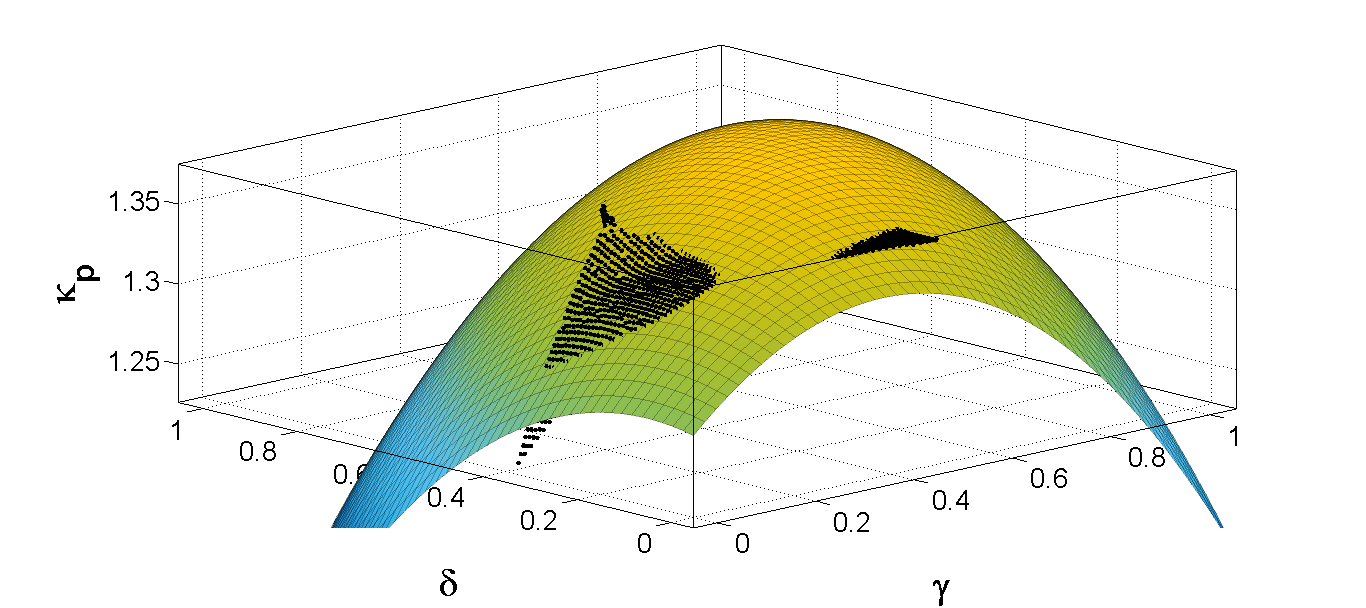
\includegraphics[width=\columnwidth]{kpfit2.png}
	\caption{Second order fit for $\kappa_p$ when $a=0.1$ and $t_{0}=1$}
	\label{F:cftoolkp}
\end{figure}
%
%\begin{figure}
%	\centering
%	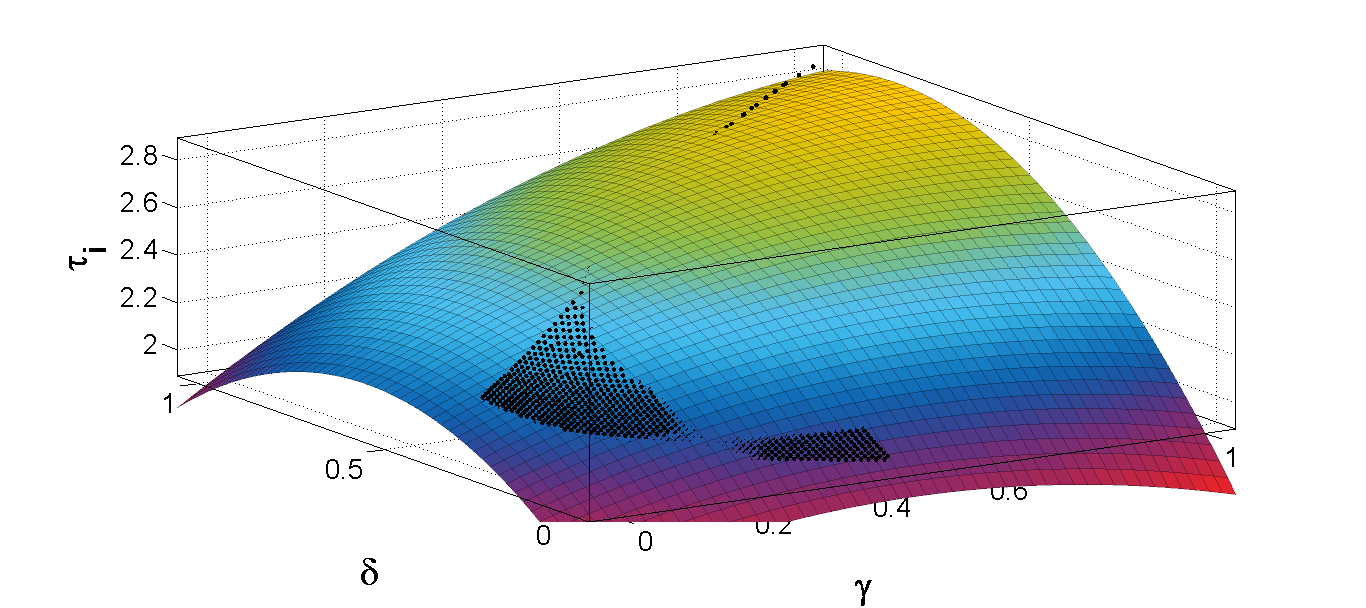
\includegraphics[width=\columnwidth]{Tifit2.png}
%	\caption{Second order fit for $\tau_i$ when $a=0.1$ and $\tau_0=1$}
%	\label{F:cftoolTi}
%\end{figure}
%
%\begin{figure}
%	\centering
%	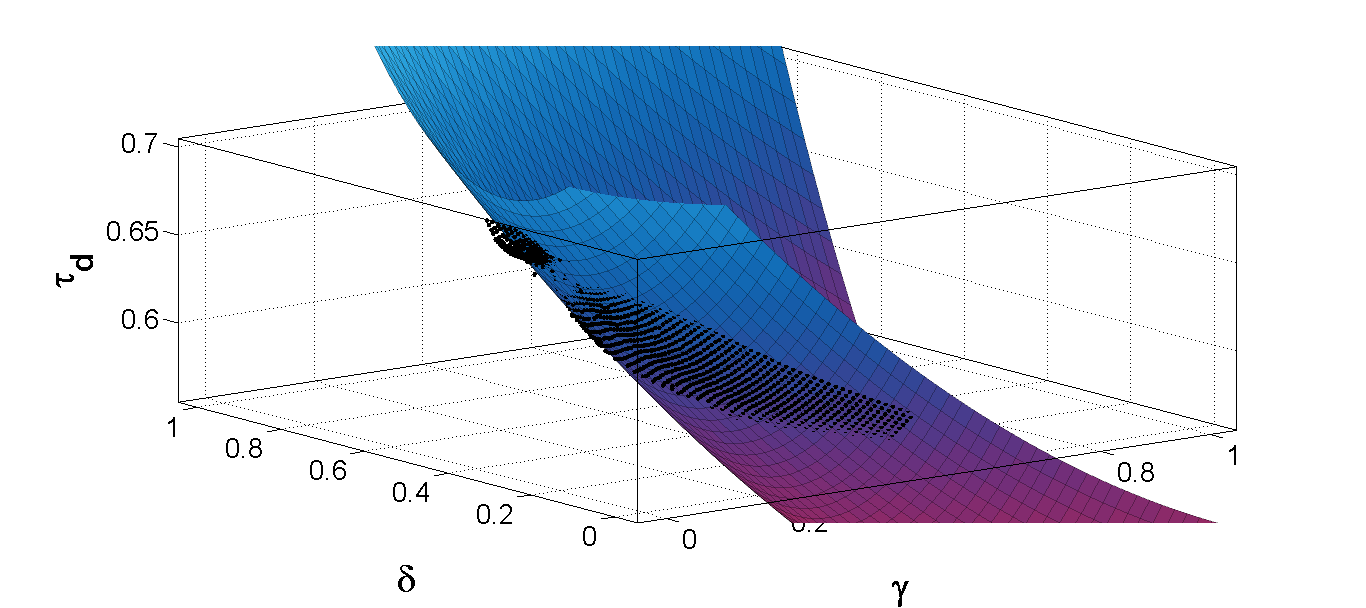
\includegraphics[width=0.5\textwidth]{Tdfit2.png}
%	\caption{Second order fit for $\tau_d$ when $a=0.1$ and $\tau_0=1$}
%	\label{F:cftoolTd}
%\end{figure}
%%
%\begin{figure}
%	\centering
%	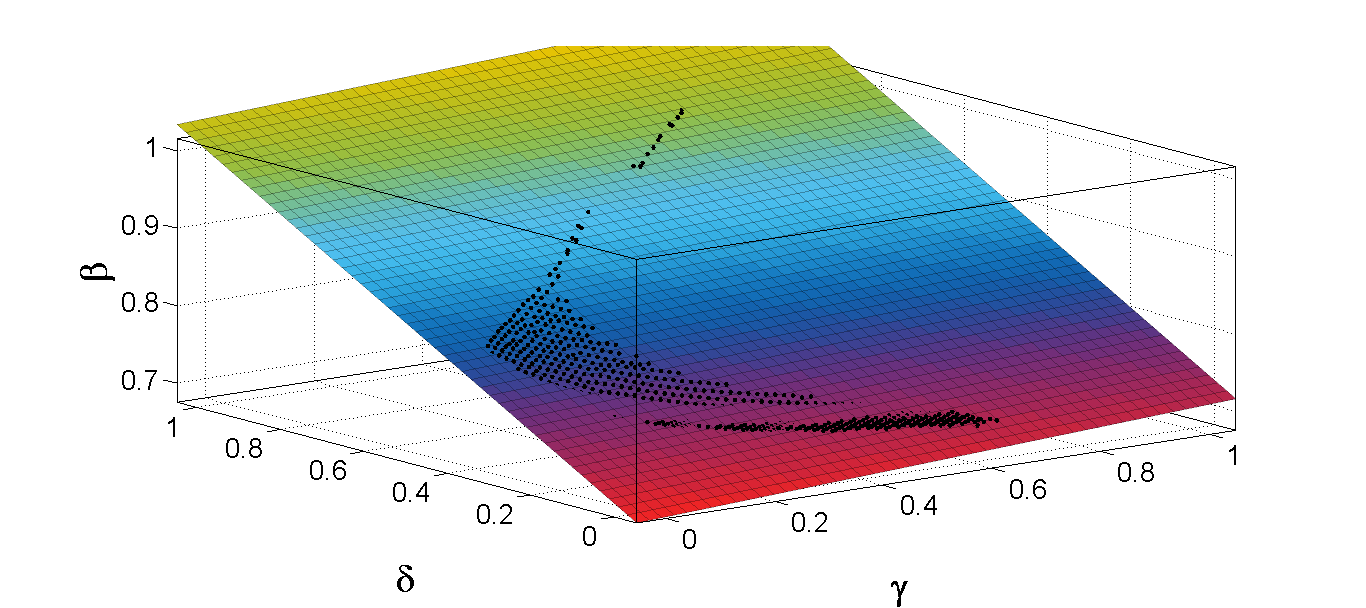
\includegraphics[width=0.5\textwidth]{betafit2.png}
%	\caption{First order fit for $\beta$ when $a=0.1$ and $\tau_0=1$}
%	\label{F:cftoolbeta}
%\end{figure}

The tuning rule for all controller parameters are proposed to be as:  
%
\begin{align}
\kappa_p &= p_{00}+p_{01}\cdot\gamma+p_{02}\cdot\delta\nonumber\\
&\quad + p_{03}\cdot\gamma^2+p_{04}\cdot\gamma\cdot \delta+p_{05}\cdot\delta^2,\label{E:eqkp}\\
%
\tau_i &= p_{10}+p_{11}\cdot\gamma+p_{12}\cdot\delta\nonumber\\
&\quad + p_{13}\cdot\gamma^2+p_{14}\cdot\gamma\cdot \delta+p_{15}\cdot\delta^2,\label{E:eqTi}\\
%
\tau_d &= p_{20}+p_{21}\cdot\gamma+p_{22}\cdot\delta\nonumber\\
&\quad+p_{23}\cdot\gamma^2+p_{24}\cdot\gamma\cdot \delta+p_{25}\cdot\delta^2,\label{E:eqTd}\\
%
\beta &=p_{30}+p_{31}\cdot\gamma+p_{32}\cdot\delta,\label{E:eqbeta}
\end{align}
%

The coefficients $p_{ij}$, where $i=\{0,1,2,3\}$ and $j=\{0,1,2,3,4,5\}$, all vary according to $a$ and $\tau_0$. This dependency suggested to perform another regressions over these parameters in terms of $a$ and $\tau_0$. Therefore a curve fitting procedure was also carried out for every $p_{ij}$. As an example of these regressions, 
%
\begin{figure}
	\centering
	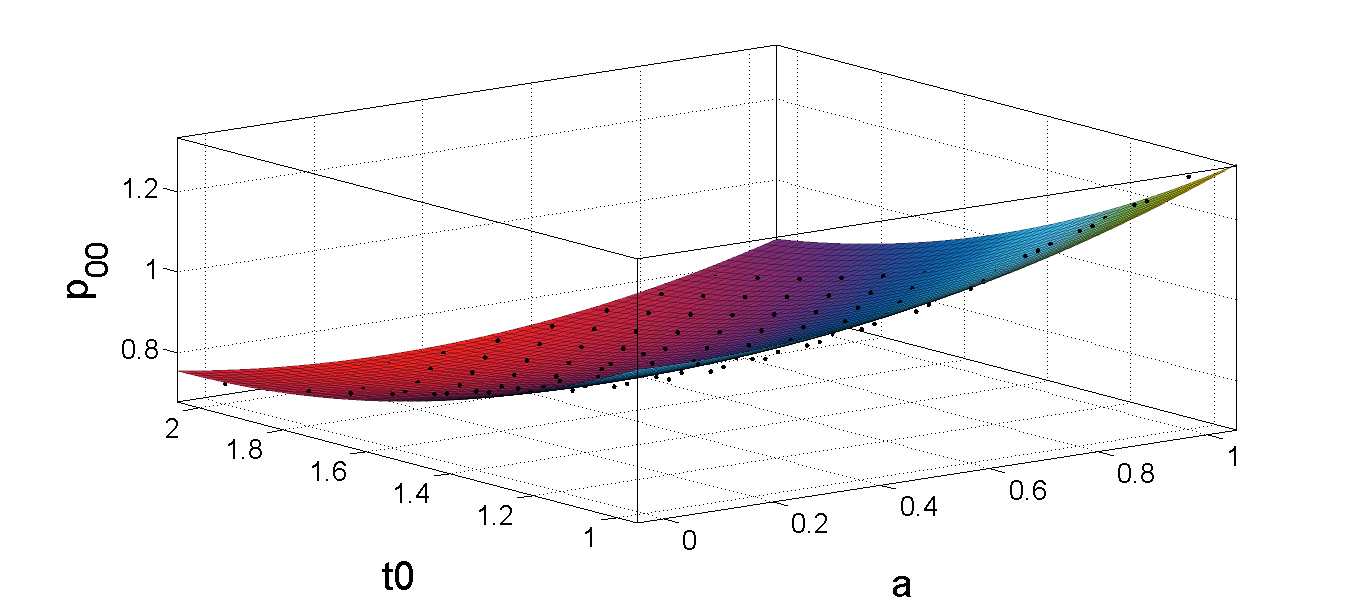
\includegraphics[width=0.8\textwidth]{./a00fit2.png}
	\caption{Second order fit for $p_{00}$ in $\kappa_p$}
	\label{F:coeff}
\end{figure}
%
Fig.~\ref{F:coeff} shows the result for the $p_{00}$ parameter as a function of $a$ and $\tau_0$.  For time-delay dominant process, the values for $\tau_0$ were considered to be in the range such that $1\leq \tau_0 \leq2$. In these cases, the adjusted R-square was higher than $0.9$. It may be possible to find a tuning equation for values of $\tau_0$ from $0.1$ to $2$ , however, this equations may become too complex to achieve a high enough adjusted R-square. This analysis is beyond the scope of this article but will be reported elsewhere.

The most appropriate fit for every coefficient in the range of $1\leq \tau_0 \leq2$, was also a second order fit. The resulting fit is described by:
%
\begin{equation}
p_{ij} = b_{i0}+b_{i1}a+b_{i2} \tau_0+b_{i3}a^2+b_{i4}a \tau_0+b_{i5}\tau_0^2 .
\label{E:coeff}
\end{equation}

Analog to $\bm{\theta}$, two hundred and twenty regressions were made for the coefficients $p_{ij}$, for every parameter in $\bm{\theta}$, except for $\beta$, which had fewer coefficients. The results of the regression analysis for every coefficient for each controller's parameter are shown in Tables~\ref{T:T1}, \ref{T:td}, \ref{T:ti} and \ref{T:beta}.

% Please add the following required packages to your document preamble:
% \usepackage{multirow}
%\begin{table}
%\centering
%\caption{Parameters for $\kappa_p$.}
%\label{T:T1}
%\begin{tabular}{|c|l|l|}
%\hline
%\multicolumn{3}{|c|}{$\kappa_p$ coefficients}           \\ \hline
%$p_{ij}$                  & \multicolumn{2}{c|}{$b_{ik}$} \\ \hline
%\multirow{6}{*}{$p_{00}$} & $b_{00}$      & 1.8203        \\ \cline{2-3} 
%                     & $b_{01}$      & 0.12765       \\ \cline{2-3} 
%                     & $b_{02}$      & -1.0484       \\ \cline{2-3} 
%                     & $b_{03}$      & 0.27085       \\ \cline{2-3} 
%                     & $b_{04}$      & -0.15141      \\ \cline{2-3} 
%                     & $b_{05}$      & 0.25505       \\ \hline
%\multirow{6}{*}{$p_{01}$} & $b_{10}$      & 0.32832       \\ \cline{2-3} 
%                     & $b_{11}$      & 0.22439       \\ \cline{2-3} 
%                     & $b_{12}$      & -0.26761      \\ \cline{2-3} 
%                     & $b_{13}$      & -0.022374     \\ \cline{2-3} 
%                     & $b_{14}$      & -0.068708     \\ \cline{2-3} 
%                     & $b_{15}$      & 0.076273      \\ \hline
%\multirow{6}{*}{$p_{02}$} & $b_{20}$      & 0.29122       \\ \cline{2-3} 
%                     & $b_{21}$      & -0.12878      \\ \cline{2-3} 
%                     & $b_{22}$      & -0.25003      \\ \cline{2-3} 
%                     & $b_{23}$      & 0.10461       \\ \cline{2-3} 
%                     & $b_{24}$      & 0.0048329     \\ \cline{2-3} 
%                     & $b_{25}$      & 0.059478      \\ \hline
%\multirow{6}{*}{$p_{03}$} & $b_{30}$      & 0.042733      \\ \cline{2-3} 
%                     & $b_{31}$      & -0.52048      \\ \cline{2-3} 
%                     & $b_{32}$      & -0.25437      \\ \cline{2-3} 
%                     & $b_{33}$      & 0.47345       \\ \cline{2-3} 
%                     & $b_{34}$      & -0.11069      \\ \cline{2-3} 
%                     & $b_{35}$      & 0.078691      \\ \hline
%\multirow{6}{*}{$p_{04}$} & $b_{40}$      & -0.077455     \\ \cline{2-3} 
%                     & $b_{41}$      & 0.61083       \\ \cline{2-3} 
%                     & $b_{42}$      & 0.24951       \\ \cline{2-3} 
%                     & $b_{43}$      & -0.60316      \\ \cline{2-3} 
%                     & $b_{44}$      & 0.19685       \\ \cline{2-3} 
%                     & $b_{45}$      & -0.071314     \\ \hline
%\multirow{6}{*}{$p_{05}$} & $b_{50}$      & -0.41226      \\ \cline{2-3} 
%                     & $b_{51}$      & -0.24733      \\ \cline{2-3} 
%                     & $b_{52}$      & 0.29554       \\ \cline{2-3} 
%                     & $b_{53}$      & 0.080236      \\ \cline{2-3} 
%                     & $b_{54}$      & 0.013411      \\ \cline{2-3} 
%                     & $b_{55}$      & -0.091089     \\ \hline
%\end{tabular}
%\end{table}
%
\begin{table}
	\centering
	\caption{Coefficients for $\kappa_p$.}
	\label{T:T1}
	\begin{tabular}{@{}cll|cll@{}}
		\hline
		%\multicolumn{6}{c}{$\kappa_p$ coefficients}           \\ \hline
		$p_{ij}$                  & \multicolumn{2}{c}{$b_{ik}$} & $p_{ij}$ & \multicolumn{2}{c}{$b_{ik}$}\\
		\hline
		\multirow{6}{*}{$p_{00}$} & $b_{00}$  & 1.820 &   \multirow{6}{*}{$p_{01}$} & $b_{10}$ & 0.328 \\ % \cline{2-3} \cline{5-6}
		& $b_{01}$      & 0.128   &  	& $b_{11}$      & 0.224 \\ % \cline{2-3} \cline{5-6}
		& $b_{02}$      & -1.048   &	& $b_{12}$      & -0.268 \\ % \cline{2-3} \cline{5-6}
		& $b_{03}$      & 0.270   &	& $b_{13}$      & -0.022 \\ % \cline{2-3} \cline{5-6}
		& $b_{04}$      & -0.151  & 	& $b_{14}$      & -0.069  \\ % \cline{2-3} \cline{5-6}
		& $b_{05}$      & 0.255   &	& $b_{15}$      & 0.076    \\ \hline
		%
		\multirow{6}{*}{$p_{02}$} & $b_{20}$  & 0.291	& \multirow{6}{*}{$p_{03}$} & $b_{30}$ & 0.043 \\ % \cline{2-3} \cline{5-6}
		& $b_{21}$      & -0.129   & & $b_{31}$      & -0.520  \\ % \cline{2-3} \cline{5-6}
		& $b_{22}$      & -0.250   & & $b_{32}$      & -0.254  \\ % \cline{2-3} \cline{5-6}
		& $b_{23}$      & 0.105    & & $b_{33}$      & 0.473   \\ % \cline{2-3} \cline{5-6}
		& $b_{24}$      & 0.005  & & $b_{34}$      & -0.111  \\ % \cline{2-3} \cline{5-6}
		& $b_{25}$      & 0.059   & & $b_{35}$      & 0.079  \\ \hline
		%
		\multirow{6}{*}{$p_{04}$} & $b_{40}$      & -0.077  & \multirow{6}{*}{$p_{05}$} & $b_{50}$      & -0.412   \\ %\cline{2-3} \cline{5-6}
		& $b_{41}$      & 0.611     &  & $b_{51}$      & -0.247\\ %\cline{2-3} \cline{5-6}
		& $b_{42}$      & 0.249     &  & $b_{52}$      & 0.296\\ % \cline{2-3} \cline{5-6}
		& $b_{43}$      & -0.603    &  & $b_{53}$      & 0.080\\ %\cline{2-3} \cline{5-6}
		& $b_{44}$      & 0.197     &  & $b_{54}$      & 0.013\\ % \cline{2-3} \cline{5-6}
		& $b_{45}$      & -0.071   &  & $b_{55}$      & -0.091\\
		\hline
	\end{tabular}
\end{table}

\begin{table}
	\centering
	\caption{Coefficients for $\tau_d$.}
	\label{T:td}
	\begin{tabular}{@{}cll|cll@{}}
		\hline
		%\multicolumn{6}{c}{$\kappa_p$ coefficients}           \\ \hline
		$p_{ij}$                  & \multicolumn{2}{c}{$b_{ik}$} & $p_{ij}$ & \multicolumn{2}{c}{$b_{ik}$}\\
		\hline
		\multirow{6}{*}{$p_{00}$} & $b_{00}$  & 0.111
		&   \multirow{6}{*}{$p_{01}$} & $b_{10}$ & -0.0076
		\\ % \cline{2-3} \cline{5-6}
		& $b_{01}$      & 0.450   &  	& $b_{11}$      & -0.163 \\ % \cline{2-3} \cline{5-6}
		& $b_{02}$      & 0.274   &	& $b_{12}$      & -0.212 \\ % \cline{2-3} \cline{5-6}
		& $b_{03}$      & -0.025   &	& $b_{13}$      & 0.154 \\ % \cline{2-3} \cline{5-6}
		& $b_{04}$      & -0.069  & 	& $b_{14}$      & -0.074  \\ % \cline{2-3} \cline{5-6}
		& $b_{05}$      & 0.003   &	& $b_{15}$      & 0.0026    \\ \hline
		%
		\multirow{6}{*}{$p_{02}$} & $b_{20}$  & -0.238	& \multirow{6}{*}{$p_{03}$} & $b_{30}$ & -0.237 \\ % \cline{2-3} \cline{5-6}
		& $b_{21}$      & 0.105   & & $b_{31}$      & -0.938  \\ % \cline{2-3} \cline{5-6}
		& $b_{22}$      & -0.016   & & $b_{32}$      & 1.121  \\ % \cline{2-3} \cline{5-6}
		& $b_{23}$      & -0.234    & & $b_{33}$      & 0.496   \\ % \cline{2-3} \cline{5-6}
		& $b_{24}$      & 0.094  & & $b_{34}$      & 0.331  \\ % \cline{2-3} \cline{5-6}
		& $b_{25}$      & -0.0254   & & $b_{35}$      & -0.641  \\ \hline
		%
		\multirow{6}{*}{$p_{04}$} & $b_{40}$      & 0.379  & \multirow{6}{*}{$p_{05}$} & $b_{50}$      & -0.224   \\ %\cline{2-3} \cline{5-6}
		& $b_{41}$      & 0.908     &  & $b_{51}$      & 0.109\\ %\cline{2-3} \cline{5-6}
		& $b_{42}$      & -1.330     &  & $b_{52}$      & 0.805\\ % \cline{2-3} \cline{5-6}
		& $b_{43}$      & -1.203    &  & $b_{53}$      & 0.669\\ %\cline{2-3} \cline{5-6}
		& $b_{44}$      & 0.215     &  & $b_{54}$      & -0.527\\ % \cline{2-3} \cline{5-6}
		& $b_{45}$      & 0.683   &  & $b_{55}$      & -0.112\\
		\hline
	\end{tabular}
\end{table}

\begin{table}
	\centering
	\caption{Coefficients for $\tau_i$.}
	\label{T:ti}
	\begin{tabular}{@{}cll|cll@{}}
		\hline
		%\multicolumn{6}{c}{$\kappa_p$ coefficients}           \\ \hline
		$p_{ij}$                  & \multicolumn{2}{c}{$b_{ik}$} & $p_{ij}$ & \multicolumn{2}{c}{$b_{ik}$}\\
		\hline
		\multirow{6}{*}{$p_{00}$} & $b_{00}$  & 0.591
		&   \multirow{6}{*}{$p_{01}$} & $b_{10}$ & -0.408
		\\ % \cline{2-3} \cline{5-6}
		& $b_{01}$      & 0.559   &  	& $b_{11}$      & 0.640 \\ % \cline{2-3} \cline{5-6}
		& $b_{02}$      & 0.545   &	& $b_{12}$      & 0.855 \\ % \cline{2-3} \cline{5-6}
		& $b_{03}$      & 0.017   &	& $b_{13}$      & -0.238 \\ % \cline{2-3} \cline{5-6}
		& $b_{04}$      & 0.045  & 	& $b_{14}$      & -0.0024  \\ % \cline{2-3} \cline{5-6}
		& $b_{05}$      & -0.028   &	& $b_{15}$      & -0.193    \\ \hline
		%
		\multirow{6}{*}{$p_{02}$} & $b_{20}$  & 1.718
		& \multirow{6}{*}{$p_{03}$} & $b_{30}$ & 1.297 \\ % \cline{2-3} \cline{5-6}
		& $b_{21}$      & 0.652   & & $b_{31}$      & -0.423  \\ % \cline{2-3} \cline{5-6}
		& $b_{22}$      & -1.160   & & $b_{32}$      & -2.095  \\ % \cline{2-3} \cline{5-6}
		& $b_{23}$      & -0.855    & & $b_{33}$      & 1.226   \\ % \cline{2-3} \cline{5-6}
		& $b_{24}$      & -0.719  & & $b_{34}$      & -1.041  \\ % \cline{2-3} \cline{5-6}
		& $b_{25}$      & 0.363   & & $b_{35}$      & 0.649  \\ \hline
		%
		\multirow{6}{*}{$p_{04}$} & $b_{40}$      & -0.077  & \multirow{6}{*}{$p_{05}$} & $b_{50}$      & -1.346   \\ %\cline{2-3} \cline{5-6}
		& $b_{41}$      & 0.621     &  & $b_{51}$      & -1.148\\ %\cline{2-3} \cline{5-6}
		& $b_{42}$      & 0.277     &  & $b_{52}$      & 1.224\\ % \cline{2-3} \cline{5-6}
		& $b_{43}$      & -1.193    &  & $b_{53}$      & -0.218\\ %\cline{2-3} \cline{5-6}
		& $b_{44}$      & 1.030     &  & $b_{54}$      & 0.512\\ % \cline{2-3} \cline{5-6}
		& $b_{45}$      & -0.025   &  & $b_{55}$      & -0.572\\
		\hline
	\end{tabular}
\end{table}


\begin{table}
	\centering
	\caption{Coefficients for $\beta$.}
	\label{T:beta}
	\begin{tabular}{@{}cll}
		\hline
		%\multicolumn{6}{c}{$\kappa_p$ coefficients}           \\ \hline
		$p_{ij}$                  & \multicolumn{2}{c}{$b_{ik}$}  \\
		\hline
		\multirow{6}{*}{$p_{00}$} & $b_{00}$  & 0.538
		
		\\ % \cline{2-3} \cline{5-6}
		& $b_{01}$      & 0.023     \\ % \cline{2-3} \cline{5-6}
		& $b_{02}$      & 0.179   	\\ % \cline{2-3} \cline{5-6}
		& $b_{03}$      & -0.114    \\ % \cline{2-3} \cline{5-6}
		& $b_{04}$      & 0.047   	  \\ % \cline{2-3} \cline{5-6}
		& $b_{05}$      & -0.034   \\ \hline
		%
		\multirow{6}{*}{$p_{01}$} & $b_{10}$  & -0.152
		\\ % \cline{2-3} \cline{5-6}
		& $b_{11}$      & 0.065    \\ % \cline{2-3} \cline{5-6}
		& $b_{12}$      & 0.277      \\ % \cline{2-3} \cline{5-6}
		& $b_{13}$      & 0.017      \\ % \cline{2-3} \cline{5-6}
		& $b_{14}$      & -0.052   \\ % \cline{2-3} \cline{5-6}
		& $b_{15}$      & -0.082     \\ \hline
		%
		
		\multirow{6}{*}{$p_{02}$} & $b_{20}$  & 0.585
		\\ % \cline{2-3} \cline{5-6}
		& $b_{21}$      & -0.082    \\ % \cline{2-3} \cline{5-6}
		& $b_{22}$      & -0.280      \\ % \cline{2-3} \cline{5-6}
		& $b_{23}$      & 0.116      \\ % \cline{2-3} \cline{5-6}
		& $b_{24}$      & 0.011   \\ % \cline{2-3} \cline{5-6}
		& $b_{25}$      & 0.044     \\ \hline
		%
		
	\end{tabular}
\end{table}
%
\subsection{Comparison of regression results vs. ENCC results}

After setting up the proposed equations for $\bm{\theta}$, simulations were run to compare the original data against the proposed methodology. The test plant is modeled as: 

\begin{equation}
P_1(s) = \frac{e^{-1.5\hat{s}}}{(\hat{s}+1)(0.5\hat{s}+1)}
\label{E:P1}
\end{equation}

Where $K=1$, $T=1$ s, $L=1.5$ s and $a = 0.5$. 
Table \ref{T:comparison} shows a comparison between the results of the tuning from the MOO problem against the results of using the proposed tuning, where the values for $\delta$ and $\gamma$ were chosen to be the worst case scenario for both $J_{do}$ and $J_{di}$, so $\delta=1$ and $\gamma=1$. 
%
\begin{table}
	\centering
	\caption{Comparison of the \gls{ennc} \gls{moo} data vs. fitted data, using $\delta = 1$ and $\gamma = 1$.}
	\label{T:comparison}
	\begin{tabular}{@{}K{0.25\columnwidth} K{0.25\columnwidth} K{0.25\columnwidth}@{}}
		\toprule
		$\bm{\theta}$ parameters and IAEs & ENCC Method & Fitted data\\
		\midrule
		$\kappa_p$	& $0.810$	& $0.793$ \\
		$\tau_i$	& $2.176$ s	& $2.113$ s	\\
		$\tau_d$	& $0.644$ s	& $0.720$ s \\
		$\beta$		& $1.000$	& $1.000$ \\
		$J_r$		& $2.689$ 	& $2.691$ \\
		$J_{di}$ 	& $2.687$ 	& $2.673$ \\
		$J_{do}$	& $2.689$	& $2.691$ \\
		$M_s$		& $1.9174$	& $1.9449$\\
		\bottomrule
	\end{tabular}
\end{table} 

As it can be seen from Table \ref{T:comparison}, results obtained from the proposed tuning rule are very similar to those obtained from the \gls{ennc} \gls{moo} method. Plots for each method were drawn as shown in Fig.~\ref{F:firstsim}.
%%%ESTA FIGURA HAY QUE CENTRARLA MEJOR
%
\begin{figure}
	\centering
	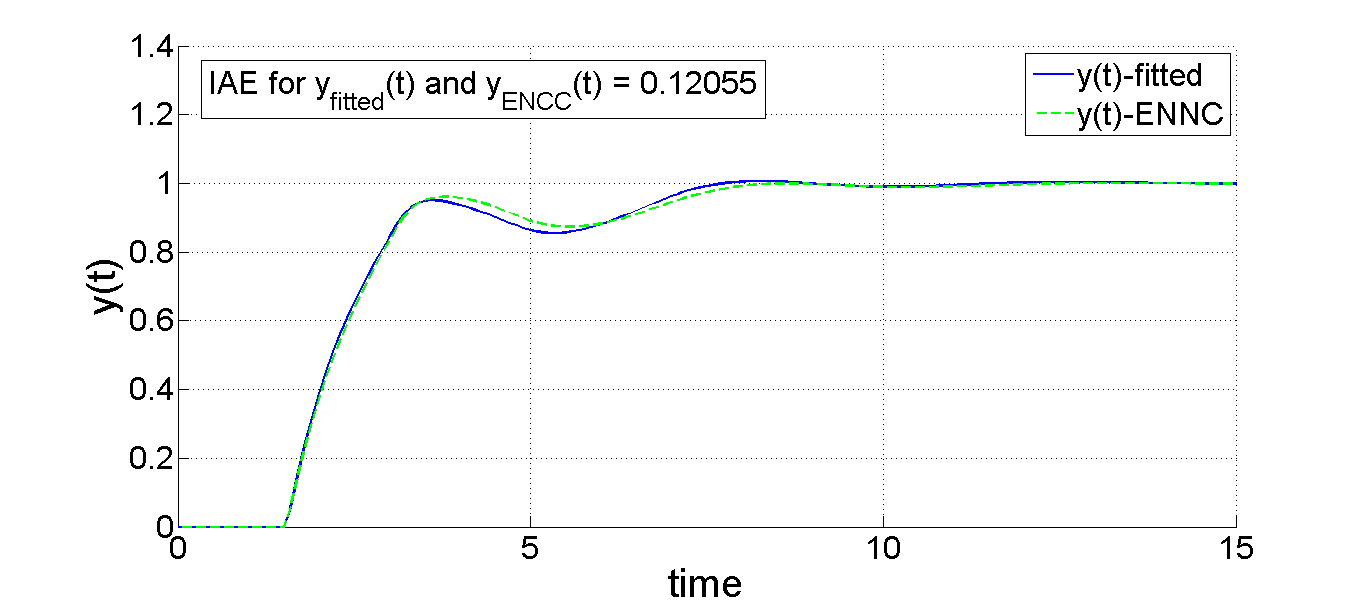
\includegraphics[width=0.8\columnwidth]{servo2.png}
	\caption{Servo response for the ENCC results and regressions results.}
	\label{F:firstsim}
\end{figure}
%
The response of the control signal is given in Fig.~\ref{F:u1}.
%
\begin{figure}
	\centering
	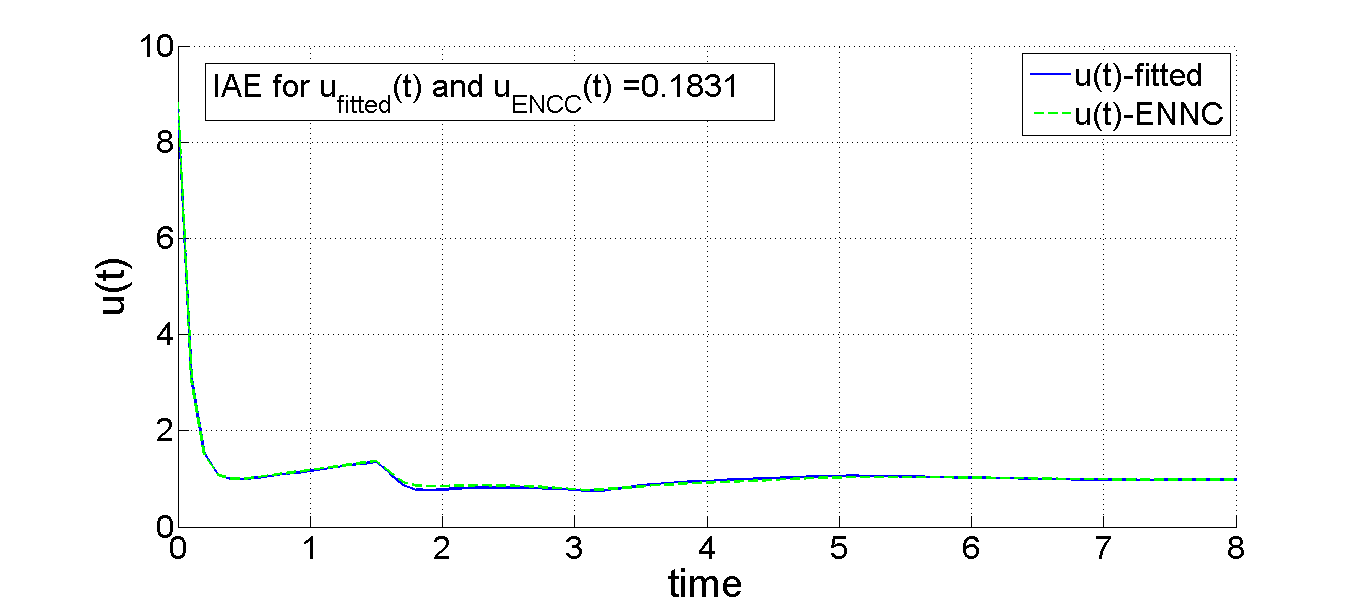
\includegraphics[width=0.8\columnwidth]{u2.png}
	\caption{Control action response for ENCC results and regressions, for a reference step change.}
	\label{F:u1}
\end{figure}

The comparison of the response to an input-disturbance is presented in Fig.~\ref{F:di1}. The error between the proposed methodology and the \gls{moo} results has an \gls{iae} of $0.08$, showing that the polynomial equations are able to encapsulate the optimal tuning of the parameters. In Fig.~\ref{F:do1}, the response to the output disturbance is presented and, as it can be seen, the match is good as well, with an \gls{iae} value of $0.12$.
%
\begin{figure}
	\centering
	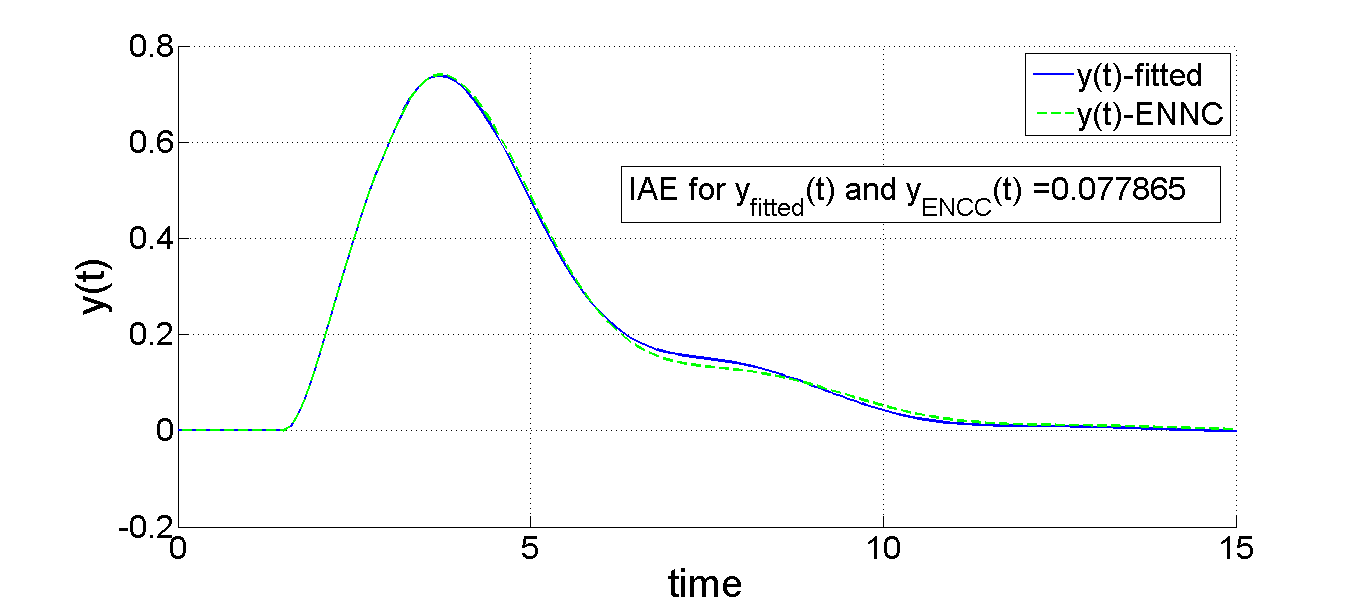
\includegraphics[width=0.8\columnwidth]{di2.png}
	\caption{Step input disturbance response for ENNC results and regressions results.}
	\label{F:di1}
\end{figure}
%
\begin{figure}
	\centering
	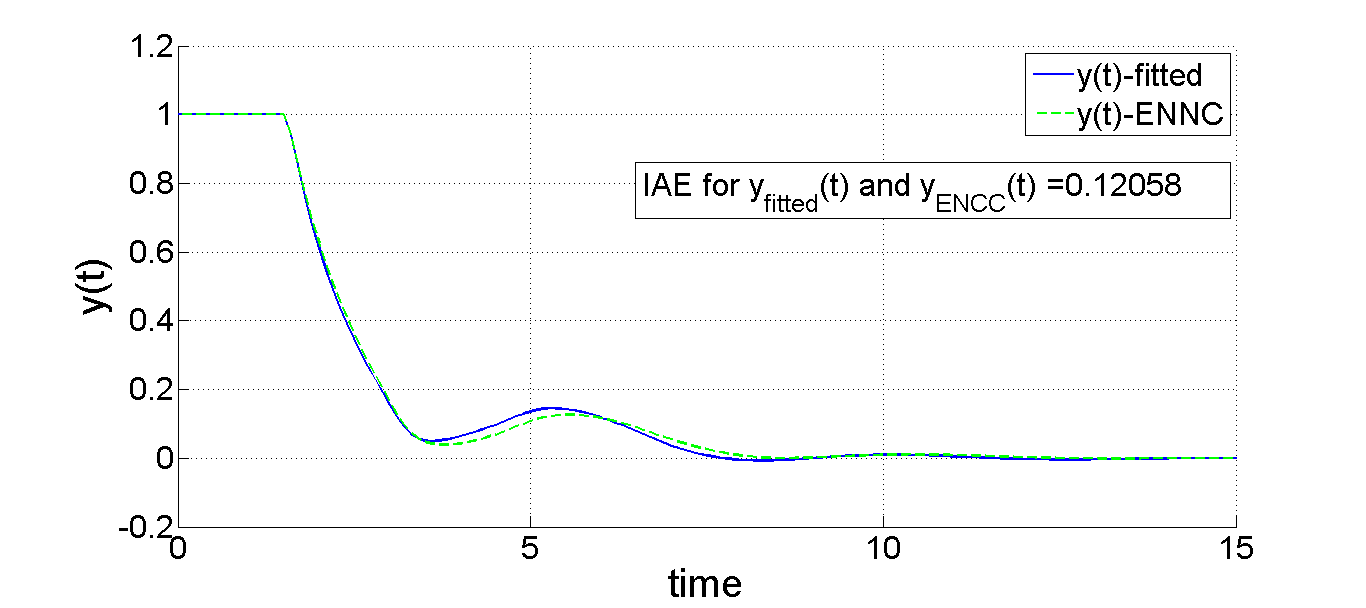
\includegraphics[width=0.8\columnwidth]{do2.png}
	\caption{Step output disturbance response for ENNC results and regressions results.}
	\label{F:do1}
\end{figure}
%

From this example, it is clear that the obtained polynomial equations effectively reproduce the behavior of the parameters found from the ENNC optimization.

The method is also tested for the extreme case scenarios for $\tau_0$ ($\tau_0=1$ and $\tau_0=2$), as given by the models:
%
\begin{equation}
P_F(\hat{s}) = \frac{e^{-\hat{s}}}{(\hat{s}+1)(0.5\hat{s}+1)},
\label{E:p2}
\end{equation}
%
\begin{equation}
P_S(\hat{s}) = \frac{e^{-2\hat{s}}}{(\hat{s}+1)(0.5\hat{s}+1)},
\label{E:p3}
\end{equation}
%
where $P_F(\hat{s})$ and $P_S(\hat{s})$ stand for the fastest and slowest time-delayed dominant test-bench plants, respectively.

For each of these plants, it was established that $\delta = 0.5$ and $\gamma = 0.5$, which is an intermediate case for degradation for both $\delta$ and $\gamma$ in the Pareto front. Results for $J_r$ for $P_F$ and $P_S$ are shown in Table \ref{T:T2}.

\begin{table}
	\centering
	\caption{Results for $J_{di}$, $J_{do}$ and $J_{r}$, using $\delta = 0.5$ and $\gamma = 0.5$.}
	\label{T:T2}
	\begin{tabular}{@{}K{0.25\columnwidth} K{0.25\columnwidth} K{0.25\columnwidth}@{}}
		\toprule
		$\bm{\theta}$ and IAE & For $P_F(s)$ & For $P_S(s)$\\
		\midrule
		$\kappa_p$	& $1.150$ 	& $0.742$ \\
		$\tau_i$ 	& $1.987$ s & $2.345$ s \\
		$\tau_d$ 	& $0.425$ s & $0.629$ s \\
		$\beta$ 	& $0.887$ 	& $0.919$ \\
		$J_r$ 		& $1.955$ 	& $3.360$ \\
		$J_{di}$ 	& $1.729$ 	& $3.162$ \\
		$J_{do}$ 	& $1.874$ 	& $3.237$ \\
		$M_s$		& $2.024$	& $1.976$ \\
		\bottomrule
	\end{tabular}
\end{table} 
%

From these examples, it is clear that the proposed methodology is able to produce Pareto-optimal controllers, for a large set of plants. The obtained dynamical response can be easily changed by the control engineer and, if the selection of $\delta$ and $\gamma$ is appropriate, the controller parameters are likely to produce a closed-loop system with a maximum sensitivity such that $M_s \leq 2$. The principal characteristic of the proposed methodology, is its ability to let the user select the dynamical behavior, taking into account multiple sources of disturbances, unlike other \gls{pid} tuning rules.

\subsection{Comparison of proposed tuning rule against uSORT2 tuning rule}
%
Servo and disturbance responses were obtained for the test-bench plant in \eqref{E:P1}, by using the proposed tuning rule, and then, by using the uSORT2 tuning method for \gls{2dof} \gls{pid} controllers. The objective is to compare both rules to see which one is more flexible in terms of robustness and performance. The uSORT2 method was selected for comparison given that it minimizes $J_{di}$ and find a sub-optimal solution for $J_r$ while keeping $M_s=2$.
%
%Three cases were considered, one in which $\delta$ and $\gamma$ were maximum as in the comparison made in Table~\ref{T:T4}, and the others were when $\delta$ and $\gamma$ have their minimum achievable value for the obtained Pareto front as in Table~\ref{T:T5} and Table~\ref{T:T6}.

Two cases were considered, one in which $\delta$ and $\gamma$ were maximum as in the comparison made in Table~\ref{T:T4}, and the others were when $\delta$ and $\gamma$ have their minimum achievable value for the obtained Pareto front as in Table~\ref{T:T5}.
%%
\begin{table}
	\centering
	\caption{Result comparison of the proposed tuning rule vs. uSORT2 tuning rule, using $\delta = 1$ and $\gamma = 1$.}
	\label{T:T4}
	\begin{tabular}{@{}K{0.25\columnwidth} K{0.25\columnwidth} K{0.25\columnwidth}@{}}
		\midrule
		$\bm{\theta}$ and IAEs & Proposed tuning rule & uSORT2 tuning rule \\
		\midrule
		$\kappa_p$ & 0.793 & 0.814 \\
		$\tau_i$ & 2.113 s & 1.676 s \\
		$\tau_d$ & 0.720 s & 0.775 s \\
		$\beta$ & 1.000 & 0.788 \\
		$J_r$ & 2.691 & 2.692 \\
		$J_{di}$ & 2.673 & 2.290 \\
		$J_{do}$ & 2.691 & 2.451 \\
		$M_{s}$ & 1.945 & 2.007 \\
		\bottomrule
	\end{tabular}
\end{table} 
%
\begin{table}
	\centering
	\caption{Comparison of the proposed tuning rule vs. uSORT2 tuning rule, using $\delta = 0.302$ and $\gamma = 0$.}
	\label{T:T5}
	\begin{tabular}{@{}K{0.25\columnwidth} K{0.25\columnwidth} K{0.25\columnwidth}@{}}
		\midrule
		$\bm{\theta}$ parameters and IAEs & Proposed tuning rule & uSORT2 tuning rule \\
		\midrule
		$\kappa_p$ & 0.820 & 0.814 \\
		$\tau_i$ & 1.808 s & 1.676 s \\
		$\tau_d$ &  0.670 s & 0.775 s \\
		$\beta$ & 0.8261 & 0.788 \\
		$J_r$ & 2.653 & 2.692 \\
		$J_{di}$ & 2.307 & 2.290 \\
		$J_{do}$ & 2.431 & 2.451 \\
		$M_{s}$ & 1.935 & 2.007 \\
		\bottomrule
	\end{tabular}
\end{table}
%%
%\begin{table}
%\centering
%\caption{Result comparative of the proposed tuning rule vs. uSORT2 tuning rule, using $\delta = 0$ and $\gamma = 0.208$.}
%\label{T:T6}
%\begin{tabular}{@{}K{0.25\columnwidth} K{0.25\columnwidth} K{0.25\columnwidth}@{}}
%\midrule
%$\bm{\theta}$ parameters and IAEs & Proposed tuning rule & uSORT2 tuning rule \\
%\midrule
%$\kappa_p$ & 0.855 & 0.814 \\
%$\tau_i$ & 1.762 s & 1.676 s \\
%$\tau_d$ &  0.604 s & 0.775 s \\
%$\beta$ & 0.763 & 0.788 \\
%$J_r$ & 2.573 & 2.692 \\
%$J_{di}$ & 2.143 & 2.290 \\
%$J_{do}$ & 2.484 & 2.451 \\
%$M_{s}$ & 1.980 & 2.007 \\
%\bottomrule
%\end{tabular}
%\end{table}
%%
%%
\begin{figure}
	\centering
	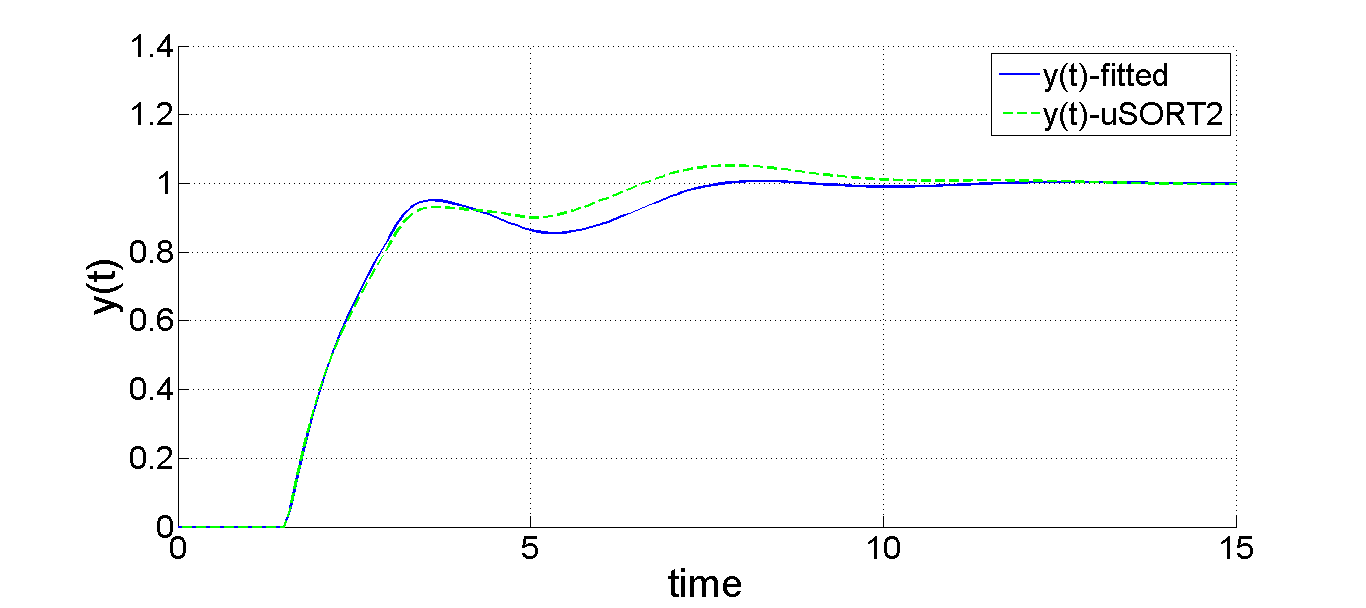
\includegraphics[width=0.8\columnwidth]{./uSORT2.png}
	\caption{Servo input response for both proposed rule and uSORT2 rule.}
	\label{F:uSort}
\end{figure}
%%
%From the results obtained in Tables \ref{T:T4}, \ref{T:T5} and \ref{T:T6},
It is clear that for the two different variations of $\delta$ and $\gamma$, the minimum \gls{iae} for servo response was obtained according to the Pareto front. Also it is important to note that, for the proposed tuning rule, although variations of $\delta$ and $\gamma$ were performed, the maximum sensitivity remained under the value of $M_s \leq 2.0$. This means that given any two inputs within the established Pareto front, the proposed tuning rule gives the optimized value for $J_r$ and it manages to maintain the controller robustness. On the other hand, the uSORT2 tuning rule only focuses on the latter. %For the three given cases in tables \ref{T:T4}, \ref{T:T5} and \ref{T:T6}, the proposed tuning rule proves to be versatile not only in terms of robustness, but also in terms of performance choice.
The uSORT2 methodology provides excellent results, but it is focused on optimizing $J_{di}$. The proposed methodology, although more complex in its equations, gives the control engineers, the freedom to mold the dynamic response to their needs. As an example, the servo response of the controlled system with the proposed methodology and the uSORT is presented in Fig.~\ref{F:uSort}
\section{MOOT-PID, multi-objetive optimization tool for PID controllers}
\label{sec:results}
%
An application that allows the user to optimally tune \gls{2dof} \gls{pid} using a \gls{soptd} model for the plant was developed. Since all the results in the obtained database are optimal from a Pareto standpoint, it is necessary to provide the user with a tool to select the final tuning of the controller.

The user has to provide the following inputs:
\begin{enumerate}
	\item A plant model in the form of a \gls{soptd} transfer function.
	\item A desired robustness (given by the maximum sensitivity).
	\item The allowed degradation of each cost function. The user can choose a degradation level from zero to one for each cost function ($J_r$, $J_{di}$, $J_{do}$). A value of zero means no degradation and one represents a total degradation. One of the cost functions needs to have a degradation of zero. If this is not true, the program automatically finds the lowest value of $J_{di}$.
\end{enumerate}
%
The tool then provides the Pareto-optimal tuning along with a simulation of the closed-loop response. It has to be noticed that the tool interpolates only from the Pareto front. Even if the user let any function to have a degradation of 1, the tuning still is Pareto optimal. Therefore, the performance of the closed loop will be better (in the Pareto sense and with the given constraints) than any other possible parameter combinations.

\subsection{Presentation of the tool}
The main window is shown in %
%
\begin{figure}%[t]%[ht]
	\centering
	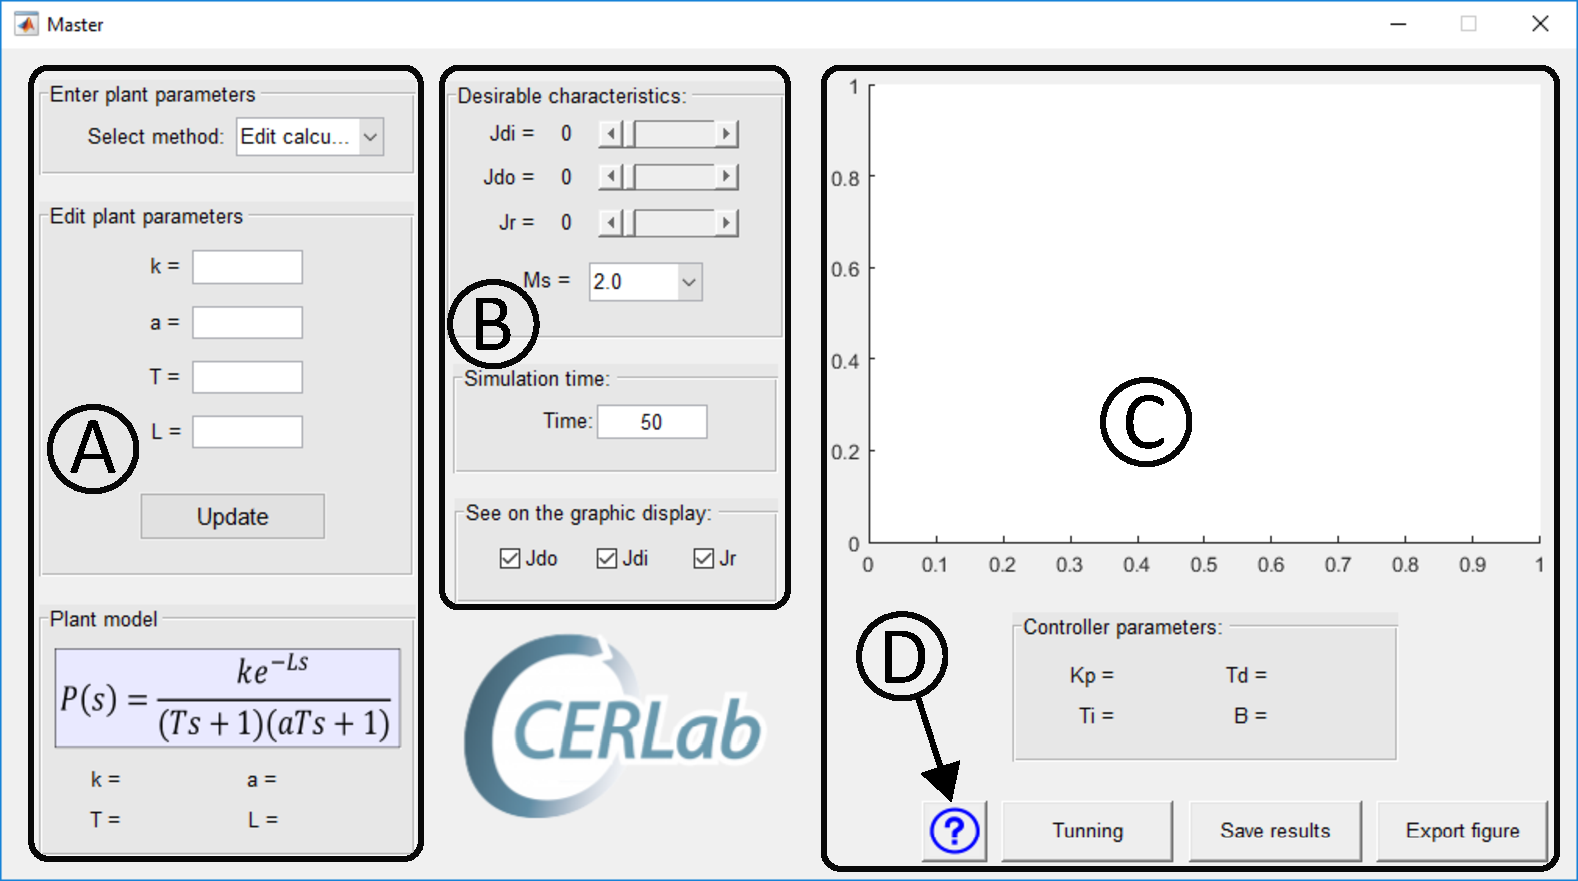
\includegraphics[width=\textwidth]{figuras/gui}
	\caption{The developed \gls{gui} for tuning \gls{pid}.}
	\label{f:gui_tuner}
\end{figure}
%
Fig~\ref{f:gui_tuner}. The \gls{gui} has four main components:
%
\begin{itemize}
	\item ``A'' part was designed to introduce the plant parameters using one of three possible methods: directly introducing its parameters, identifying the model plant from workspace data or identifying a plant model from a comma-separated values (CSV) file. These options are selected in the left top corner of the \gls{gui}.
	\item ``B'' part allows to choose the desirable characteristics for the tuning of a \gls{2dof} \gls{pid}, using the degradation values of $J_{di}$, $J_{do}$ and $J_r$. Also, the closed-loop robustness can be selected by the variable $M_S$.
	\item ``C'' part where the results of ``A'' and ``B'' parts are shown, in graphical and numerical form. It is possible to generate a report of results in plain text format and also to export the generated figure to \matlab.
	\item The ``D'' part is the help manual, that explains the steps for using the \gls{gui}.
\end{itemize}
%

As it can be seen, the user interface is simple and easy to use. Since all the optimization have been performed off-line, the tool is fast in finding the final tuning. The simulation of the closed-loop was computed with a MEX compiled file that solves the delay differential equations\footnote{Compiled MEX files are provided for 64 bits Linux and Windows machines. Other architectures or operating systems should be compiled from source.} using a fourth order Runge-Kutta algorithm.

% \begin{figure}
% \begin{center}
% \includegraphics[width=0.45\textwidth]{figuras/diagrama_proceso}
% \caption{Operating scheme.}
% \end{center}
% \end{figure}
%
\subsection{Plant model}
To model the plant, either from the workspace or from a CSV file, there are two possible ways to find the parameters of the \gls{soptd} method. The first method is using the 123-C algorithm, that uses three points of the reaction curve to find the model~\parencite{Alfaro2006}. The other method uses the optimization toolbox to find the best parameters of the \gls{soptd} transfer function.

The tool was tested by applying an experimental identification of a \gls{soptd} plant described by
\begin{equation}
P(s)=\frac{e^{-0.2s}}{(s+1)(0.5s+1)}.
\label{e:test1}
\end{equation}

The input data correspond to an artificial response produced using \eqref{e:test1}. From the data, the results using the optimization method for system identification presented in %
%
\begin{figure}%[ht]
	\begin{center}
		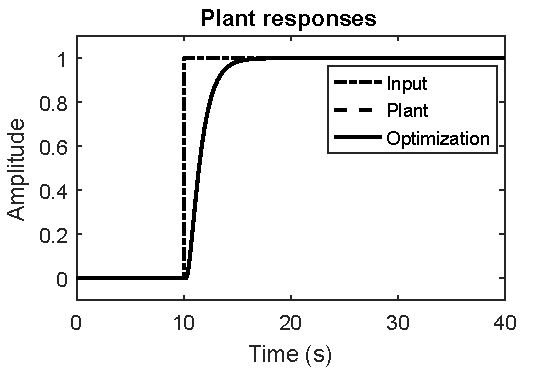
\includegraphics[width=0.65\columnwidth]{figuras/identification}
		\caption{Operating scheme.}
		\label{f:test_res_1}
	\end{center}
\end{figure}
%
%
Fig.~\ref{f:test_res_1}. As it can be seen, the programmed optimization was able to find exactly the model of the plant. It is very important to count with a good model since the interpolation performed in the tool depends heavily from the knowledge of the parameters. The tool is able to find the \gls{pid} controller if the following conditions on the plant are fulfilled:
\begin{equation}
\begin{split}
0.1 &\leq \frac{L}{T} \leq 2 \\
0 &\leq a \leq 1
\end{split}
\label{eq:limits}
\end{equation}
%
\subsection{Example of use.}
\label{sec:example}
%
The \gls{soptd} plant in \eqref{e:test1} is used to verify the correct operation of this tool. A typical closed-loop response is presented in %
\begin{figure}
	\centering
	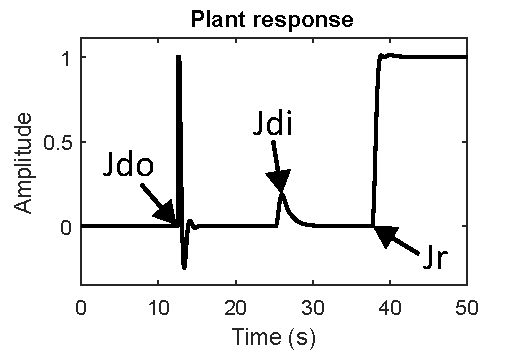
\includegraphics[width=0.65\columnwidth]{figuras/tuning}
	\caption{Control loop response given by the tool.}
	\label{f:control_loop_response}
\end{figure}
Fig~\ref{f:control_loop_response}. As it can be seen, the tool is able to plot the response of each cost function individually.

In order to demonstrate the usefulness of the tool, three different scenarios where tested. On %
%
\begin{table}
	\centering
	\caption{Degradation of parameters.}
	\label{t:jdi_jdo_jr_deg}
	\begin{tabular}{cccccc}
		\toprule
		\multicolumn{1}{c}{\textbf{Parameter}} & \textbf{Figure} & \textbf{Jdi} & \textbf{Jdo} & \textbf{Jr} & \textbf{Ms} \\
		\midrule
		$J_{di}$                      & Fig.~\ref{f:jdi_comp}  & 0.1/0.9      & 0.5          & 0           & 2.0         \\
		$J_{do}$                     &    Fig.~\ref{f:jdo_comp}& 0            & 0.1/0.9      & 0.5         & 2.0         \\
		$J_r$                      &   Fig.~\ref{f:jr_comp} & 0            & 0.5          & 0.1/0.9     & 2.0         \\
		\bottomrule
	\end{tabular}
\end{table}
%
Table~\ref{t:jdi_jdo_jr_deg} the degradation settings are shown. Each case represents the change in the response where one degradation is changed while the others are kept constant. In all cases one of the cost functions degradation is set to zero, this means that, from all the possible optimal tuning that fulfills the degradation requirements, the tool is going to give the tuning that produces the lowest cost function for that particular cost function. When the user selects the desired levels of degradation that do not correspond to the Pareto front (that is, a point so close to the utopia point that does not correspond to the feasible region), a pop-up window appears asking the user to relax the degradation limits.

On %
\begin{figure}
	\begin{center}
		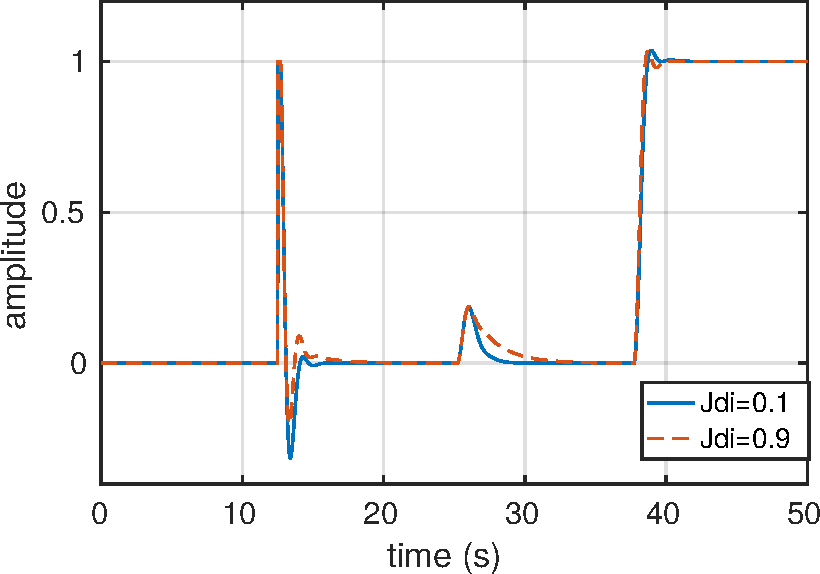
\includegraphics[width=0.65\columnwidth]{figuras/jdi_comp}
		\caption{Variation of $J_{di}$ degradation while keeping the other degradations constant.}
		\label{f:jdi_comp}
	\end{center}
\end{figure}
Fig.~\ref{f:jdi_comp}, two different responses are shown where the allowed degradation of $J_{do}$ is changed while maintaining the other parameter constant. The first response corresponds to a change in $d_o(s)$, the second one is a change in $d_i(s)$ and the final response is a change in $r(s)$. It is clear that, when allowing a higher degradation of $J_{di}$, the response to $d_i(s)$ has a larger \gls{iae}. However, since the responses to each disturbance sources are not independent, varying one degradation settings makes the other responses to vary. However, since the degradation of $J_r$ was kept constant at zero, the tuning given by the tool correspond to the lower value of $J_r$, while satisfying the other degradation levels.

The response of the second case of Table~\ref{t:jdi_jdo_jr_deg} is presented in %
\begin{figure}
	\centering
	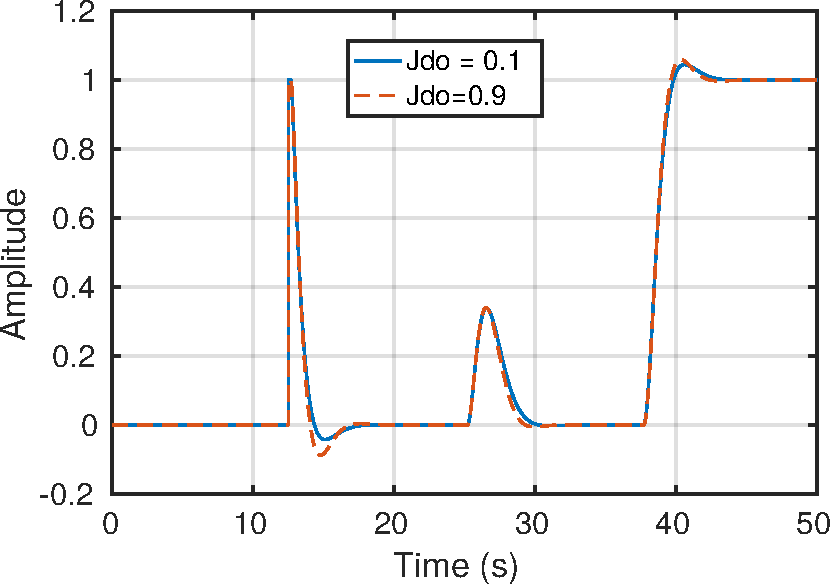
\includegraphics[width=0.65\columnwidth]{figuras/jdo_comp}
	\caption{Jdo comparison.}
	\label{f:jdo_comp}
\end{figure}
%
Fig.~\ref{f:jdo_comp}. This case is interesting because it reflects one of the benefits of analyzing the tuning of \gls{pid} parameters using the Pareto framework. It is clear that, from the point of view of the control engineer, the tuning with a degradation of $J_{do}=0.1$ is more advantageous than for the case of $J_{do}=0.9$, because the degradation on the other responses is minimal while improving the response to a change in $d_o(s)$. Finding this results is easy using the tool presented in this paper, without the need to perform individual optimization for each case.

The third case is presented in %
\begin{figure}
	\centering
	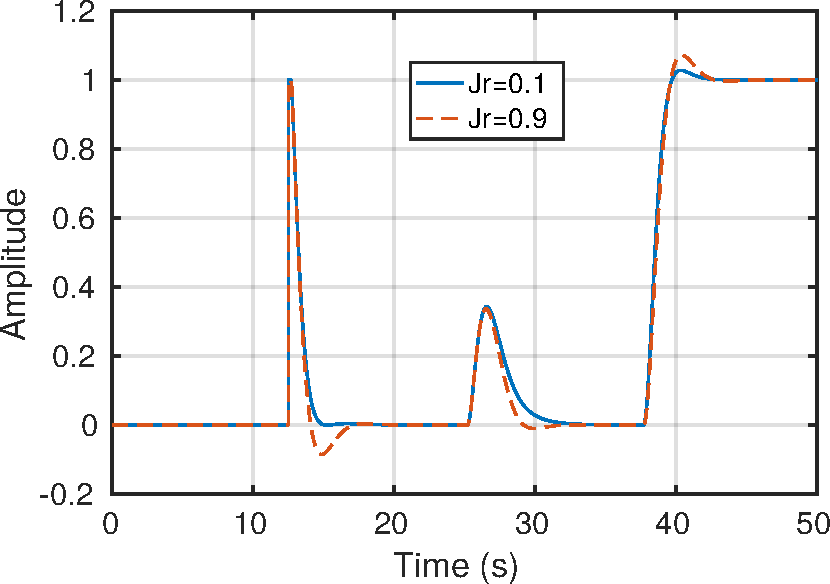
\includegraphics[width=0.65\textwidth]{figuras/jr_comp}
	\caption{Jr comparison.}
	\label{f:jr_comp}
\end{figure}
%
Fig~\ref{f:jr_comp}. In this case is interesting to note that when the allowed degradation of $J_r$ is set to $0.1$, the performance of input disturbance rejection response is also improved. This is important to note because, even thought all three cost function has some kind of antagonism, there are some sections of the Pareto front where is possible to improve two function at the cost of worsening the third function as in this case. The tuning of all the controllers are presented in
%
\begin{table}
	\caption{Obtained parameter of the presented cases.}
	\label{tab:Tunings}
	\centering
	\begin{tabular}{cccccc}
		\toprule
		Case & value & $K_p$ & $T_i$ & $T_d$ & $\beta$\\
		\midrule
		\multirow{2}{*}{$J_{di}$} & $0.1$ & $4.8874$ & $1.1198$ & $0.2566$ & $0.6111$\\
								  & $0.9$ & $4.7449$ & $2.0346$ & $0.2809$ & $0.9095$ \\
		\midrule
		\multirow{2}{*}{$J_{do}$} & $0.1$ & $1.6891$ & $1.2225$ & $0.2738$ & $0.7322$\\
								  & $0.9$ & $1.7400$ & $1.1333$ & $0.2255$ & $0.6647$\\
		\midrule
		\multirow{2}{*}{$J_{r}$}  & $0.1$ & $1.7237$ & $1.4461$ & $0.2522$ & $0.8874$\\
								  & $0.9$ & $1.7166$ & $1.0971$ & $0.2535$ & $0.6685$\\
		\bottomrule
	\end{tabular}
\end{table}
%
Table~\ref{tab:Tunings} for reference. Finally, the last characteristic of the tool is that it is able to save the results of the tuning in plain text. An example of the output report is %
%
\begin{figure}
\centering
\begin{tcolorbox}
%\small
\begin{verbatim}
Characteristic,Value
Plant parameters,Value
K,1
T,1
a,0.5
L,0.2
Desirable characteristics,Value
Jdi,0.26
Jdo,0.24
Jr,0
Ms,2.0
Controller parameters,Value
Kp,4.7206
Ti,1.3629
Td,0.2848
B,0.7379
\end{verbatim}
\end{tcolorbox}
%\normalsize
\caption{Report output.}
\label{f:report_tuning}
\end{figure}
%
presented in Fig.~\ref{f:report_tuning}.
\printbibliography
\end{refsection}

\backmatter%%%%%%%%%%%%%%%%%%%%%%%%%%%%%%%%%%%%%%%%%%%%%%%%%%%%%%%
%\Extrachap{Glossary}
%\printglossaries
%\include{solutions}
%\printindex

%%%%%%%%%%%%%%%%%%%%%%%%%%%%%%%%%%%%%%%%%%%%%%%%%%%%%%%%%%%%%%%%%%%%%%

\end{document}





